
\chapter{Imitation vs. Innovation - \newline Die Wirkung einer Exportunterstützung auf den technologischen Entwicklungsstand eines Landes}\label{Papier1}
\chaptermark{Innovation vs. Imitation}


In Kapitel \ref{sec:Globalisierung} wurden einige historische Industrialisierungsprozesse vorgestellt, die deutliche Unterschiede in ihrer Auspr{\"a}gung gezeigt haben. Zum einen bez{\"u}glich der Entwicklungsgeschwindigkeit eines Landes, dem industriellen Wachstum, zum anderen hinsichtlich der Organisations- und Produktionsstrukturen, die in einer Vielschichtigkeit von Institutionen m{\"u}ndeten \citep{Gerschenkron.1962}.\\


Der Blick in die Vergangenheit hat gezeigt, dass auch heute das globale Wachstumspotenzial noch nicht ausgeschöpft ist, was vor allem auf die relativ weniger weit entwickelten L{\"a}nder zurück zu führen ist. Das von den Aufholprozessen der Entwicklungsl{\"a}nder die gesamte Weltwirtschaft profitieren wird, prognostizierte die Weltbank in ihrem j{\"a}hrlichen Entwicklungsbericht von 2013. Das zuk{\"u}nftige globale Wachstum wird dabei nicht auf das Wachstum der Industriel{\"a}nder zur{\"u}ckgef{\"u}hrt, sondern ma{\ss}geblich von der Entwicklung weniger weit entwickelter Volkswirtschaften abh{\"a}ngen. \newline Der Aufholprozess der Entwicklungsl{\"a}nder spielt jedoch nicht nur beim Wirtschaftswachstum eine gro{\ss}e Rolle, sondern auch bei dem Anstieg des Handelsvolumens. So sollte sich innerhalb von vier Jahren, also von 2012 bis 2015, das Handelsvolumen von 3,5{\%} auf 7{\%} verdoppeln, was sich jedoch leider nicht bewahrheitet hat (Datenbank Weltbank).\\


Zu beobachten ist eine Welt mit globalen Wissensstr{\"o}mungen unabh{\"a}ngig von L{\"a}ndergrenzen. Jedes Wirtschaftssubjekt kann von der Welttechnologiegrenze profitieren und dadurch den lokalen Wissensstand verbessern. Dies kann auf zweierlei Arten geschehen, durch Innovation oder Imitation. Es ist zu beobachten, dass in einigen L{\"a}ndern das Wachstum verst{\"a}rkt aus imitativen T{\"a}tigkeiten hervorgeht. Diesem Zusammenhang, vor allem in Hinblick auf Offenheit eines Landes, wird sich im folgenden gewidmet. Dabei wird im vorliegenden Modell neben dem Einflussfaktor Au{\ss}enhandel der Einfluss des technischen Fortschritts auf den Entwicklungsprozess untersucht. Diese Modellvariation basiert auf der Arbeit von \citet{Acemoglu.2006}, die den technischen Fortschritt endogen modelliert haben und somit nicht durch externe Wissenseffekte bedingt ist. Technischer Fortschritt kann hier auf zwei Arten entstehen: entweder durch Innovation oder durch Imitation. Je nachdem wie sich zunächst einzelne Unternehmen und letztlich die gesamte Volkswirtschaft entscheiden, folgen sie der Imitaions- oder Innovatiosstrategie. \\


In ihrem Modell schildern \citet{Acemoglu.2006}, dass L{\"a}nder von einer aktiven Regierung profitieren k{\"o}nnen. Durch den zielgerichteten Einsatz der staatlichen Lenk- und Leitungsfunktion kann ein Aufholprozess angeregt werden. Weniger entwickelte L{\"a}nder können technisches Wissen aufarbeiten bis sie sogar den Wissenstand der Welttechnologiegrenze erreichen. Dies schildert ein Beispiel Chinas. Es kam zwischen der Regierung Chinas und dem Gro{\ss}unternehmen Airbus zu einer detailliert geplanten Zusammenarbeit. Es wurde vertraglich festgehalten, dass mit der Auftragserteilung von Gro{\ss}projekten die Produktion dieser Maschinen in China selbst stattfinden sollte. Dadurch reduzierte sich nicht nur die Arbeitslosigkeit im Land, sondern führte zus{\"a}tzlich zu einem technologischen Wissenszuwachs {\"u}ber die Herstellung moderner Flugzeuge. Die staatliche Zusammenarbeit mit verschiedenen Gro{\ss}unternehmen wie Airbus zielt darauf ab, komplette Produktionszweige in das eigene Land zu holen und dadurch den Technologietransfer aktiv zu f{\"o}rdern.\\


Das Beispiel verdeutlicht lediglich, dass Au{\ss}enhandel und damit verbundene staatliche Eingriffe  das Wirtschaftswachstum fördern. Neben dem technologischen Entwicklungsstand eines Landes beeinflusst auch Handel die strategische Entscheidungsfindung in diesem Modell. Schlie{\ss}lich soll der Blick auf offene Volkswirtschaften es erlauben, eine Aussage über die Eignung und den Einfluss einer Strategie auf den jeweiligen Entwicklungsstand eines Landes treffen zu können. Da die Wahl einer Strategie auch qualitativ  beurteilt werden kann, sollten mit ihrer Hilfe auch Empfehlungen für offene Länder mit einem bestimmten Entwicklungsstand möglich werden. 
Handel und eine damit verbundene Exportunterst{\"u}tzung fördert vor allem den Entwicklungsprozess eines weniger weit entwickelten Landes. Ähnlich wie China durch den Import von Technologien einen höheren technologischen Entwicklungsstand im Bereich der Luftfahrt erreichen konnte, soll hier die Modellierung einer Exportförderung ebenfalls zum Aufholprozess eines Landes beitragen. Es wird gezeigt, dass es f{\"u}r diese Entwicklungsl{\"a}nder ratsam ist, sich auf die Imitation von Produkten zu konzentrieren und erst durch die Durchführung kleiner Projekte ihren Wissensstand erh{\"o}hen. Erst dann sollte die Innovation neuer Produkte oder Produktionstechniken angestrebt werden. Die zentralen Fragen lauten: Welche Auswirkungen hat Au{\ss}enhandel auf den technologischen Entwicklungsstand eines Landes? Ist die Exportunterst{\"u}tzung entscheidend f{\"u}r die Wahl einer Imitations- oder Innovationsstrategie? Im wesentlichen wirkt sich Au{\ss}enhandel durch die in Kapitel \ref{Effekte Handel} beschriebenen Effekte positiv auf den technologischen Entwicklungsstand aus und bedingt die Wahl der Strategie.
Jedoch haben noch weitere Faktoren Einfluss auf die Strategiewahl, wie z.B. die Auswahl des Managers der für die technische Ausrichtung des Unternehmens zuständig ist.\footnote{\citet{Acemoglu.2006} gehen vor allem auf die Qualifikationen der Führungskräfte hinschlich des Kerngeschäfts eines Unternehmens, der Produktentwicklung, ein, damit werden vor allem die technischen Fähigkeiten betont. Deshalb wird in der folgenden Arbeit der englischsprachige Begriff des "`entrepreneu"'s mit Ingenieur übersetzt, in der Funktion der technischen Geschäftsführung bzw. des Leiters der Forschungs- und Entwicklungsabteilung.} Die Unternehmen selbst haben die Möglichkeit ihre Führungskräfte gezielt auszutauschen und damit indirekt die Strategie zu bestimmen. Auf makroökonomischer Ebene ergibt sich dabei eine Unternehmensstruktur die zur Innovations- oder Imitationsstrategie tendiert. 
Es wird angenommen, dass die Innovationsstrategie, sowie die damit verbundene Wahl des technischen Geschäftsführers wichtiger wird, je mehr sich ein Land der Welttechnologiegrenze (WTG) nähert. Indem die Beziehung zwischen dem Abstand zur WTG und der Forschungs- und Entwicklungsintensit{\"a}t analysiert wurde, konnte diese Annahme von \citet{Griffith.2004} best{\"a}tigt werden. Dafür wurde zunächst die Lage zur WTG bestimmt, die durch den Quotient aus der totalen Faktorproduktivit{\"a}t im Verh{\"a}ltnis zur weltweiten totalen Faktorproduktivit{\"a}t, jeweils eines industriellen Sektors, beschrieben wird. Die Aufwendungen f{\"u}r Forschung und Entwicklung stellen das Ma{\ss} f{\"u}r die Intensit{\"a}t dieser dar. Es ergibt sich ein signifikant positiver Zusammenhang zwischen beiden Gr{\"o}{\ss}en. Forschungs- und Entwicklungsinvestitionen sind also bedeutender f{\"u}r L{\"a}nder die einen relativ geringen Abstand zur Welttechnologiegrenze aufweisen \citep{Acemoglu.2006}.\newline
Die folgende Analyse unterscheidet anders als \citet{Acemoglu.2006} zwischen Makro- und Mikroinnovationen, um den Wirkungsrahmen einer Innovation zu berücksichtigen \citep{Mokyr.1990}. Dadurch soll noch deutlicher hervorgehoben werden, dass nicht jede Innovation eines Landes den Weltmarkt beeinflusst, jedoch trotzdem den Entwicklungsprozess beeinflussen kann. Dies bedingt jedoch verschiedene Formen der WTG, die im folgenden differenziert werden.


\sectionmark{WElttechnologiegrenze}
\section{Die Welttechnologiegrenze als Bezugsgrö{\ss}e}\label{WTG}
\sectionmark{WElttechnologiegrenze}


Es wird angenommen, dass das Land, welches den höchsten Wissensstand in einer Weltwirtschaft verkörpert, die Welttechnologiegrenze $\overline {A}_t$ vorgibt. Der technologische Knowhow-Stand eines jeweils betrachteten Landes wird dabei durch das produktivste Unternehmen mit der am weitesten entwickelten Technologie definiert. 
Neben diesen Annahmen basiert auch das folgende Konzept überwiegend auf dem Aufsatz von \citet{Acemoglu.2006}. Es wird angenommen, dass sich der Entwicklungsstand eines Landes am Abstand zur Welttechnologiegrenze (WTG) bemisst. Bevor jedoch der Abstand zur WTG genauer betrachtet wird, muss die WTG genauer beleuchtet werden. Grundsätzlich gilt hierbei:
\begin{equation}\overline{A}_t=\overline{A}_0(1+g)^t\label{exogene WTG}\end{equation}
Ausgehend von einem fiktiven Anfangsbestand $\overline{A}_0$ wächst der technische Fortschritt über die Zeit $t$ konstant mit der Rate $g$.\\ 


Dabei werden zwei verschiedene Ansätze berücksichtigt. Zum einen kann es sich um eine \textsl{exogen} gegebene Welttechnologiegrenze handeln. In diesem Fall sind mikroökonomische Innovationen für den Rest der Welt nicht relevant. Zum anderen kann sich die Technologiegrenze \textsl{endogen} weiterentwickeln, wodurch sich ein weltweiter Wirkungskreis der Innovationen ergibt, in diesem Zusammenhang ist von makroökonomischen Innovationen die Rede.\footnote{Die Terminologie der zu unterscheidenden Innovationen geht auf \citet{Mokyr.1990} zurück und es wird im Folgenden zwischen mikroökonomischen Innovationen technologisch kleiner Länder und makroökonomischen Innovationen technologisch gro{\ss}er Länder unterschieden.}


\subsection{Exogene Welttechnologiegrenze}\label{sec:exogene WTG}
Die WTG ist bei technologisch kleinen Ländern exogen. Hierbei sind technologisch kleine Länder von ökonomisch kleinen Ländern zu unterscheiden. Ein technologisch kleines Land kann Innovationen entwickeln, die die Produktivität dieses Landes erhöhen. Dies ist jedoch in relativ weiter entwickelten Länder nicht zwingend. Es hängt von der "`Reichweite"' bzw. dem Wirkungskreis einer Innovation ab. Ähnliche Länder würden demnach zwar von einer solchen Innovation profitieren, jedoch hat dies keine Auswirkungen auf das technologisch am weitesten entwickelte Land, das die Technologie an der WTG bereitstellt.\\


Die Neuerung an einer Nähmaschine, beispielsweise ein besserer Nähfu{\ss} für Rei{\ss}verschlüsse, wird zwar die Produktivität eines Landes erhöhen, welches sich auf die Textilindustrie spezialisiert hat, aber nicht zu einer Ausweitung der Welttechnologiegrenze führen. Demnach ist es dem betrachteten Land nicht möglich selbst die WTG zu bilden, indem es neue Technologien erfindet, die diese erweitern. Das technologisch kleine Land hat, bei ansonsten gleichen Bedingungen, ein technisches Wachstum, welches langfristig gegen die WTG konvergiert und darin enden kann.
Mikroökonomische Innovationen und Skaleneffekte beeinflussen die WTG nicht, da deren Auswirkungen zu gering sind und sie nur in dem Land selbst, jedoch nicht weltweite Folgen mit sich bringen. Die hier beschriebene Technologiegrenze entspricht der in Gleichung \eqref{exogene WTG} dargestellten WTG mit einer exogenen Wachstumsrate $g$. 
Unterscheiden sich die Einflussgrö{\ss}en der betrachteten Volkswirtschaft von der technologisch führenden Volkswirtschaft, dann konvergiert der Entwicklungsstand des Landes nicht zwingend zur WTG. Deutlich schlechtere Bedingungen im Land führen dazu, dass der maximal erzielbare Zustand nicht erreicht werden kann. Auf diese Problematik wird in Kapitel \ref{sec:Wirkung von Handel auf das technologisch kleine Land} näher eingegangen. 


\subsection{Endogene Welttechnologiegrenze} \label{sec:endogene WTG}
Eine WTG ist endogen, wenn eine Innovation auf diese Einfluss nehmen kann. Der technische Fortschritt äu{\ss}ert sich hier bei der Produktion der Zwischengüter. Kommt es in einem Zwischengutsektor zu einer makroökonomischen Innovation, welche die WTG langfristig erweitert, dann handelt es sich um ein technologisch gro{\ss}es Land.
\begin{equation}\overline{A}_t=\overline{A}_0(1+g_j)^t\end{equation}
Die Wachstumsrate des technischen Fortschritts $g_j$ ist endogen. Somit weitet sich die Welttechnologiegrenze mit jeder zusätzlichen Innovation aus. Als Beispiel dient eine technologische Revolution der letzten Jahrzehnte: das Internet. Diese Innovation hat die WTG ausgeweitet und Einfluss auf die Produktivität vieler Einsatzfaktoren, Branchen und Länder gehabt. Jegliche operative Prozesse im Unternehmen wurden optimiert. Allein der Einkauf und Vertrieb von Produkten kann nun effizienter durchgeführt werden. Um auf das vorangegangene Beispiel zurück zu kommen, wurde in der Textilindustrie der Bezug von Stoffen und Material vereinfacht und ebenso der Verkauf gefertigter Produkte. Es erleichtert dem Konsumenten, die Vielfalt der Produkte wahrzunehmen und steigert dadurch  die Wohlfahrt eines Landes \citep{Krugman.79}.\\


Dies bedeutet jedoch nicht, dass von den makroökonomischen Innovationen technologisch gro{\ss}er Länder auch jedes Land profitieren kann. Gerade für technologisch weniger weit entwickelte Länder ist die Ausweitung der WTG nicht so bedeutend. Es ist noch nicht die gesamte Welt durch das Internet miteinander verbunden, auch wenn es theoretisch möglich wäre. In afrikanischen Ländern wie beispielsweise Ghana ist die technische Infrastruktur rudimentär ausgebaut und es bestehen sehr hohe Verbindungskosten, die den Nutzen übersteigen. Eine Nutzung des Internets ist dann ökonomisch nicht sinnvoll. Auch politische Ma{\ss}nahmen wie die Zensur bestimmter Internetseiten schränkt die Nutzung ein.\\


Hier ist bei einer endogenen WTG entscheidend, dass per Annahme jedes Land bzw. Unternehmen zu jeder Technologie Zugang hat und mit einer makroökonomischen Innovation die WTG beeinflusst.


\bigskip
Da sich der Abstand zur WTG an der relativen Lage der lokalen Technologiegrenze zur WTG der Vorperiode bemisst, gilt: $\frac{\overline{A}_{t-1}}{A_{t-1}}$. Nachdem die WTG $\overline{A}_{t}$ genauer definiert wurde, wird für die Betrachtung des Entwicklungsstandes noch die lokale Technologiegrenze (LTG) eines Landes benötigt, die im Folgenden erläutert wird.



\subsection{Lokale Technologiegrenze}
Das technologisch am weitesten entwickelte Land repräsentiert die WTG. Der produktiv\-ste Sektor stellt den technologischen Wissensstand des Landes dar. Der Entwicklungsstand eines Sektors wird wiederum durch das produktivste Unternehmen des Sektors abgebildet. 
In jedem Sektor gibt es eine technologische Höchstgrenze. Demzufolge unterscheiden sich die technologischen Entwicklungsstände eines Landes pro Sektor. In dem vorliegenden Modell gibt es nur zwei Sektoren, jedoch unendlich viele Zwischengüter. Wird eine Innovation erfolgreich entwickelt, kann es zum Wechsel des führenden Unternehmens eines Sektors kommen, sofern es sich nicht um eine Innovation des bereits führenden Unternehmens handelt. Diese Innovation führt überregional entweder zum technologischen Aufholen eines Landes oder zur Ausweitung der Welttechnologiegrenze, wenn es bereits führend war. Das Überspringen des technologisch am weitesten entwickelten Landes wird ausgeschlossen.\\
Ist eine Innovation nicht erfolgreich, dann verbleibt eine Volkswirtschaft auf dem bisherigen technologischen Entwicklungsstand. Unter der lokalen Technologiegrenze $A_t$ ist demzufolge der technologische Entwicklungsstand eines Landes zu verstehen. Die Technologiegrenze eines Landes wird somit durch das am weitesten entwickelte Unternehmen eines Landes beschrieben, welches die höchste Produktivität aufweist.\\ 


Die Beurteilung der Produktivität kann erst nach eingehender Untersuchung des theoretischen Modells vorgenommen werden. In diesem Zusammenhang wird auch der Abstand der LTG zur WTG definiert.



\sectionmark{Produktion}
\section{Produktion der Unternehmen}\label{sec:Produktion}
\sectionmark{Produktion}
Das vorliegende Modell orientiert sich weiterhin an dem Model von \citet{Acemoglu.2006}. Es basiert auf dem multisektoralen, schumpeterianischen Modell, welches bereits in Kapitel \ref{sec:schumpeter} beschrieben wurde und den technischen Fortschritt im Zwischengutsektor ansiedelt, wodurch die Entwicklung von Innovationen weniger zufällig, sondern kalkulierbar wurde. Es wird allerdings um einen weiteren Endproduktsektor erweitert, damit zu einem späteren Zeitpunkt ein zweites Gut existiert, mit dem Handel betrieben werden kann und eine Handelsstruktur bestimmt werden kann. Zunächst wird jedoch nur ein Endproduktsektor betrachtet.\\
Das Endprodukt wird von einem Monopolisten eins zu eins für die Herstellung einer Einheit eines Zwischengutes genutzt. Das jeweilige finale Gut wird also für die Produktion von Zwischengütern eingesetzt, die gleichzeitig auch Einsatzfaktoren für das Endprodukt sind. Jedoch geht der Produktionsfaktor Zwischengut in geringerem Ma{\ss}e in die Endproduktproduktion ein, sodass ein Rest an Endprodukten bleibt, der konsumiert oder für Forschungszwecke reinvestiert werden kann.\footnote{Ein Endprodukt kann direkt in ein Zwischenprodukt umgewandelt werden. Die Produktionselastizität des Zwischengutes $\alpha$ ist jedoch kleiner 1. Demnach wird weniger als eine Einheit des Zwischengutes benötigt, um eine Einheit des Endproduktes herzustellen. Es entsteht ein Rest an Endprodukten.}\\


In den betrachteten Volkswirtschaften entscheiden sich die Unternehmen zwischen der Innovations- oder der Imitationsstrategie. Innovationen entstehen ausschlie{\ss}lich in den Zwischengutsektoren, in denen demnach der technische Fortschritt wiederzufinden ist. Bei der technologischen Innovation kann es sich sowohl um die Entwicklung neuer Güter bzw. Zwischengüter, als auch um neue Herstellungsverfahren und Prozesse handeln. Bei der Imitation von Gütern oder Produktionsmechanismen stehen allen Unternehmen die neuesten und am weitesten entwickelten Technologien zur Verfügung.\\


Das Modell, in dem die Lebensdauer der Wirtschaftssubjekte zwei Perioden beträgt und die Zukunft mit dem Zinssatz $r$ diskontiert wird ist Generationen-überlappend. Die Bevölkerung setzt sich zusammen aus Arbeitern und einem Ingenieur. Demnach beläuft sich die Bevölkerungsgrö{\ss}e auf $N+1$. Es wird davon ausgegangen, dass die Bevölkerung  nicht wächst und somit konstant bleibt. Die Bevölkerung wird hälftig unterteilt in die Kapitalisten als die Anteilseigner des Unternehmens und Arbeiter. Die Kapitalisten haben lediglich die Eigentumsrechte inne, aber ansonsten keine weitere operative Funktion und können bezüglich des Produktionsprozesses vernachlässigt werden. Die Eigentumsrechte werden innerhalb von Dynastien häufig vererbt und es besteht für Au{\ss}enstehende keine Möglichkeit, diese anderweitig zu erlangen.\\


Die Arbeiter sind mit handwerklichen und unternehmerischen, hier technischen Fähigkeiten ausgestattet. Sie besitzen zwar die gleiche handwerkliche Begabung, unterscheiden sich jedoch in der Produktivität bei den Aufgaben hinsichtlich Forschung und Entwicklung. Die unternehmerischen Fähigkeiten sind je nach Bildungsstand mit der Wahrscheinlichkeit $\lambda$ hoch oder mit $(1-\lambda)$ gering.\\


Es gilt für beide Bevölkerungsgruppen, dass sie gleicherma{\ss}en kein Vermögen besitzen können.



\subsection{Annahmen der Produktionsfunktion}\label{sec:Annahmen der Produktionsfunktion}
Die Produktion eines Endprodukts, welches gleichzeitig für die Produktion von Zwischengütern benötigt wird, erfolgt unter vollständigem Wettbewerb. 
\begin{equation}y_j=\frac{1}{\alpha_j}N_{tj}^{1-\alpha_j}\left(\int_0^1{A_t(\nu)^{1-\alpha_j}x_{tj}(\nu)^{\alpha_j}}d\nu\right)\label{Produktionsfunktion} \qquad \text{mit} \qquad  j= 1;2\end{equation} 
Gleichung \eqref{Produktionsfunktion} bildet die Technologie eines Endproduktsektors ab.\footnote{Dabei gilt für das aggregierte Einkommen $y=y_1+y_{2}$. Beide Sektoren unterscheiden sich durch $\alpha_1>\alpha_{2}$. Dies wird auf den folgenden Seiten genauer erläutert.} Diese Form der Produktionsfunktion ist notwendig, um den technologischen Fortschritt endogen darstellen zu können.\\


Das Integral beschreibt das Kontinuum an Zwischengütern, das für die finale Produktion benötigt wird. Bei $x(\nu)$ handelt es sich um die Menge der Zwischengüter $\nu$, die zum Zeitpunkt $t$ für die Herstellung des Endprodukts benötigt werden. $A_t(\nu)$ ist der Produktivitätsparameter des Zwischengütersektors. Dieser modelliert hier den technischen Fortschritt, der sich wie alle weiteren fehlenden Erläuterungen bezüglich der Produktionsfunktion im folgenden Abschnitt anschlie{\ss}t.



\subsubsection{Technischer Fortschritt}
Modelle, die endogenes technologisches Wachstum darstellen, berücksichtigen eine Wahl- möglichkeit für die Wirtschaftssubjekte zwischen verschiedenen Technologien bzw. die Möglichkeit der Weiterentwicklung dieser. Investitionen in Forschung und Entwicklung führen zu einer höheren Innovationsquote. Demnach besteht hier ein positiver Zusammenhang zwischen Innovationen und Investitionen. Doch der Entstehungsprozess neuer Technologien wird häufig nicht berücksichtigt. Dieser Prozess wird in theoretischen Modellen nicht immer explizit ausformuliert. Dann wird davon ausgegangen, dass die Entdeckung und Entwicklung in der Natur der Sache von Innovationen liegt und im deterministischen Sinne nicht denkbar ist. Es sei nicht möglich, noch unbekannte Neuerungen durch eine Funktion zu beschreiben, bei der Inputfaktoren zu einem regelmä{\ss}igen Output führen.\\


In der vorliegenden Arbeit wird jedoch davon ausgegangen, dass es eine zwischengelagerte Produktionsfunktion für den technologischen Entwicklungssektor gibt, eine Art Meta-Produktions- funktion.


	\begin{equation}
		I=\lambda\gamma A_{t-1}(\nu)
	\end{equation}\label{Meta}


Diese gibt an, wie und mit welchen Einsatzfaktoren neue Technologien $I$ entstehen. Demnach werden in Volkswirtschaften Innovationen zielgerichtet entwickelt und die Kreativität kann "`produziert"' werden. Die Einsatzfaktoren sind die lokale Produktivität der vergangenen Periode $A_{t-1}(\nu)$ und die innovativen Fähigkeiten der Unternehmer $\gamma$.\footnote{Genauer gesagt handelt es sich bei $\gamma$ um einen Produktivitätsparameter bezüglich der Innovationsintensität, der angibt, wie stark sich die Technologie verändert und wie stark, mit $\gamma>1$, der neue Monopolist dem vorherigen überlegen ist.} Dabei ist jedoch ein gewisser Grad an Ungewissheit $\lambda$ zu berücksichtigen. Der Erfolg des Innovationsprozesses ist per se unsicher. Auch die Markteinführung und Annahme einer neuen Produktqualität durch den Konsumenten sind zunächst nicht vorhersehbar. Wird den Individuen per Annahme erlaubt, Kalkulationen bezüglich dieser unsicheren Faktoren vorzunehmen, aus denen eine Entscheidung hervorgeht, dann lässt sich der Prozess des technologischen Fortschritts auch in einer Modellwelt darstellen.\\
Das Gut eines Sektors wird aus Zwischengütern und aus dem Faktor Arbeit hergestellt. Gemä{\ss} der Produktionsfunktion \eqref{Produktionsfunktion} bedarf es zum Zeitpunkt $t$ für die Produktion des Endprodukts $N$ Arbeiter. Aufgrund der Erweiterung um einen zweiten Endproduktsektor ist eine Unterscheidung beider Güter erforderlich, welche im Produktionsprozess liegt. Die aggregierten Produktionsfunktionen beider Sektoren unterscheiden sich durch ihre Produktionselastizitäten, $\alpha_1>\alpha_2$. Das Endprodukt in Sektor 1 wird demzufolge mit einer höheren Intensität von Zwischengütern hergestellt, als es in Sektor 2 der Fall ist. Sektor 2 hingegen produziert das Endprodukt arbeitsintensiv und benötigt relativ wenig Zwischengüter. \\


Die Intensität der Einbindung bzw. die Anzahl der Zwischenprodukte $\nu$ in dem Produktionsprozess wird durch $x(\nu)$ abgebildet. Bei $ A_t(\nu)$ handelt es sich um die Produktivität zum Zeitpunkt $t$. Beide Sektoren verwenden die gleichen Zwischengüter, bedienen sich der gleichen Technologie und demnach resultiert auch die gleiche Produktivität. Die folgende Gleichung zeigt, dass der technische Fortschritt in der Produktivität eines Zwischengutsektor wiederzufinden ist. 

	\begin{equation}
		A_t(\nu)=s_t(\nu)[\eta\overline{A}_{t-1}+\gamma A_{t-1}(\nu)]\label{Produktivitat}
	\end{equation}

Die Produktivität eines Zwischengutes hängt unter anderem von der Projektgrö{\ss}e $s_t(\nu)$ ab. Handelt es sich um ein gro{\ss}es Projekt, dann ist $s_t(\nu)=1$. Bei einem kleinen Projekt ist $s_t(\nu)=\sigma$, mit $\sigma<1$.
Der zweite, in eckigen Klammern stehende Faktor bildet die Einflussfaktoren der jeweiligen Strategie ab. Bei dem ersten Summanden $\eta\overline{A}_{t-1}$ handelt es sich um den Anstieg der Produktivität, der durch die Nachahmung bereits vorhandener Produkte bedingt ist. Das weltweite technologische Wissen der letzten Periode ist bekannt und kann nun mit einer Intensität $\eta$ imitiert werden. Der Produktivitätsparameter $\eta$ beschreibt die Produktivitätssteigerung durch die Nachahmung von Technologien der vorherigen WTG. Bei der Nachahmung von Prozessen und Gütern kann das Wissen der WTG angewendet werden. Der zweite Summand $\gamma A_{t-1}(\nu)$ beschreibt den Prozess der Neuentwicklung von Produkten und Prozessen. Das momentan vorhandene technologische Wissen zum Zeitpunkt der Vorperiode, die LTG, kombiniert mit den Fähigkeiten des Unternehmers $\gamma$ führen zu einer Entwicklung von Innovationen. \\


Nur ein Unternehmen jedes Zwischengutsektors hat zunägst Zugang zu der produktivsten Technologie.
Dabei handelt es sich um das Pionier-Unternehmen, welches eine Innovation entwickelt und dadurch das technische Wissen des Landes ausdehnt.  Demzufolge kann es als einziges Unternehmen ein benötigtes Zwischengut herstellen und besitzt Monopolmacht.\footnote{Alle anderen Unternehmen können mit etwas Verzögerung ebenfalls die am weitesten entwickelte Technologie nutzen und das Gut imitieren, jedoch ist dies mit höheren Kosten verbunden und mindert dadurch die Konkurrenzfähigkeit.} In jedem Zwischengutsektor $\nu$ gibt es nur ein führendes Unternehmen mit Monopolmacht. Auch dieses bietet einem Arbeiter an, das technische Management des Unternehmens zu übernehmen und für das Unternehmen tätig zu werden. Nur ein technisch qualifizierter Unternehmer ist also in einem Zwischengutsektor für die technologische Entwicklung  und Ausrichtung verantwortlich.\newline
In dem betrachteten Modell wird demnach der technische Fortschritt bei der Produktion der Zwischengüter generiert, deren Markt durch monopolistische Konkurrenz gekennzeichnet ist. Jeder einzelne führende Anbieter eines Zwischengutes hat Monopolmacht inne, die jedoch durch substitutive Merkmale und Ausprägungen anderer Zwischengüter eingeschränkt ist. Ohne die monopolistische Marktform einer Branche würde der Anreiz fehlen, Innovationen zu entwickeln.
\subsubsection{Monopolistische Konkurrenz und Limit-Preis}\label{sec:LimitPreis}
Der folgende Abschnitt stellt die Notwendigkeit der monopolistischen Konkurrenz als Marktform im Zwischengutsektor und die Erfordernis eines Limit-Preises dar.\\


Ausgehend von einem Nash-Gleichgewicht \footnote{Ist in der Spieltheorie angesiedelt und beschreibt das Marktgleichgewicht, das bei sozialen Grenzkosten-Preisen liegt. Erhöht ein Marktteilnehmer den Preis, würden die Konsumenten das Gut bei den übrigen Konkurrenten zu dem geringeren Preis nachfragen. Siedelt ein Anbieter den Preis unter den Grenzkosten, mit der Absicht an, die komplette Nachfrage auf sich zu ziehen, entstehen Verluste, weil die Kostendeckung nicht gewährleistet ist. Folglich bleibt der Preis beim sozialen Grenzkosten-Preis.} können Innovationen zu monopolistischer Konkurrenz führen. Das Modell monopolistischer Konkurrenz geht zurück auf die Arbeit von \citet{Dixit.1977}. Im allgemeinen Fall der vollkommenen Konkurrenz ermöglichen Innovationen einem Anbieter, die gesamte Nachfrage auf sich zu ziehen ohne dabei Verluste zu erwirtschaften. Handelt es sich um eine Produktinnovation, die vor allem auf die Qualität des Produktes abzielt, wäre ein höherer Gewinn bedingt durch einen höheren Preis denkbar. Das Alleinstellungsmerkmal des Gutes rechtfertigt vor den Verbrauchern den höheren Preis und steigert deren Zahlungsbereitschaft. Eine Prozessinnovation mindert die Grenzkosten und dies ermöglicht dem Produzenten, seine Konkurrenten im Preiswettbewerb zu unterbieten. Hierbei sind jedoch zwei mögliche Ausprägungsformen der Prozessinnovation zu unterscheiden:  eine drastische Innovation und eine nicht-drastische Innovation.\\


Handelt es sich um eine \textit{drastische} Innovation, liegt der neue mögliche Monopolpreis unter den Grenzkosten der übrigen Mitstreiter. Der innovierende Anbieter erhält Monopolmacht und schöpft die gesamtwirtschaftliche Nachfrage in diesem Markt ab.\\


In diesem Modell wird jedoch von \textit{nicht-drastischen} Innovationen ausgegangen. Der aus der Innovation resultierende Monopolpreis zu geringen Grenzkosten ist hier grö{\ss}er, als der ursprüngliche  Grenzkosten-Preis der konkurrierenden Anbieter. Das innovierende Unternehmen kann jedoch das Zwischengut zu einem marginal geringeren Preis anbieten, einem Limit-Preis. Alle anderen Produzenten werden aus dem Markt gedrängt und der Vorreiter hat Monopolmacht. \\




Da eine Innovation in diesem Sinne die Eigenschaft der Nicht-Ausschlie{\ss}barkeit besitzt, kann die neue Technologie auch von allen weiteren Unternehmen verwendet und imitiert werden.\footnote{Dies ist jedoch mit Kosten verbunden. Der Zugang zu der neuen Technologie muss zum Limit-Preis erworben werden.} Der Wettbewerbsvorteil durch die Neuerung ist deshalb nur von kurzer Dauer und zwar solange, bis es auch allen anderen Anbietern möglich ist, zu den neuen geringen Grenzkosten zu produzieren. Hinzu kommt, dass die Kosten für die Forschung und Entwicklung der Innovation durch den Erstentwickler getragen werden. Wie auch schon von \citet{Schumpeter.1934} bestätigt, führt vollkommener Wettbewerb nicht unweigerlich zu einer Entwicklung von Innovationen, weil die Anreize zu gering sind. Laut Schumpeter ist das Streben nach Monopolmacht gleich dem Anreiz, Innovationen zu entwickeln. Ein umstrittener Markt kann durch die Entwicklung von Innovationen dominiert werden, so dass das Pionier-Unternehmen den monopolistischen Gewinn abschöpft.  In einem bereits bestehenden monopolistischen Wettbewerb ist ein Anbieter jedoch kaum motiviert, eine Innovation zu entwickeln. Er kann bereits die monopolistische Preis-Mengen-Kombination anbieten und er würde die Innovation oder die neue Technologie lediglich durch eine weiterentwickelte ersetzten.\footnote{Dabei handelt es sich um den Arrow replacement effect \citep{Arrow.1962}. Ein Anbieter hat einen geringeren Anreiz eine Innovation zu entwickeln, wenn er bereits Monopolmacht besitzt.} Die konkurrierenden Produzenten hingegen haben eine deutlich höhere Motivation, eine Innovation zu entwickeln, um dadurch letztlich den amtierenden Monopolisten ersetzen zu können. Schumpeter bezeichnete diesen Prozess als schöpferische Zerstörung, der auch als ein Motor des Wachstums gilt.\\


Innovationen führen nur dann langfristig zur Monopolmacht, wenn Unternehmen einen geschützten Zugang zur besseren Technologie als ihre Mitstreiter haben. Eine Möglichkeit besteht in der Einführung von Patenten, denn somit wäre das Pionier-Unternehmen der Innovation der alleinige Nutzer und könnte langfristig Gewinne erwirtschaften. Au{\ss}erdem lie{\ss}e sich gezielt Einfluss auf die Verbreitung seines technischen Wissens nehmen. \\


Diese Möglichkeit wird im vorliegenden Modell als die Imitation von vorherigen Innovationen beschrieben. Das Anliegen, eine geschützte Technologie zu imitieren, kann durch die Zahlung eines Limit-Preises erfolgen. Der Limit-Preis schützt den Vorreiter vor der kostenlosen Adaption neuer Entwicklungen durch die Konkurrenten und wirkt im Grundprinzip wie ein Patent.
Für die nachahmenden Unternehmen ist der jeweilige Limit-Preis auf den Zwischengütermärkten der Faktorpreis. Dies erklärt ein genauerer Blick auf die Produktionsstruktur der Zwischengüter: Für die Produktion der Zwischengüter sind die Endprodukte wiederum Einsatzfaktoren. Die adaptiven Unternehmen zerlegen das Endprodukt in seine früheren Bestandteile bis hin zu den Zwischenprodukten. \\


Die Nachahmung ist mit hohen Kosten verbunden, weil die Unternehmen anfangs eine Vielzahl von Endprodukten auseinanderbauen müssen, um das Zwischengut herstellen zu können. Die Produzenten zahlen dem Vorreiter den Limit-Preis $\chi_j$, um Zwischengüter zu erhalten. Dieser gibt die Menge bzw. Wertigkeit der Endprodukte an, die notwendig ist, um eine Einheit eines Zwischenguts zu reproduzieren. Der Limit-Preis ist auch sehr nützlich, um den Konkurrenzdruck zu parametrisieren. Je höher die Produktionskosten sind und je mehr Versuche ein Unternehmen benötig, um das Zwischengut selbst herzustellen, desto weniger umstritten ist der Markt. Der Faktorpreis bzw. Limit-Preis $\chi_j$ drückt somit indirekt die Markteintrittsbarriere und Wettbewerbsbeschränkung in einem Zwischengutsektor aus. Der limitierende Preis eines Monopolisten ist demnach formal 


	\begin{equation}
		p_{tj}(\nu)=\chi_j \label{Grenzproduktentlohnung}
	\end{equation}


Der Monopolpreis $p_{tj}$ entspricht im Marktgleichgewicht dem Grenzprodukt des Zwischengutes gemä{\ss} der Grenzproduktivitätsentlohnung.\footnote{Erfolgt durch die Ableitung von \eqref{Produktionsfunktion} nach dem Zwischengut $x_{tj}(\nu)$.}

	\begin{equation}
		\chi_j=\left(\frac{A(\nu)N_{tj}}{x_{tj}(\nu)}\right)^{(1-\alpha_j)}
	\end{equation}


Die Notwendigkeit des Limit-Preises per se wurde bereits diskutiert. Im folgenden Absatz geht es um die Höhe des Limit-Preises $p_{tj}$  bzw. innerhalb welcher Schranken sich dieser befindet. Rein intuitiv ist das imitierende Unternehmen weniger produktiv als das Pionier-Unternehmen, denn dieses Unternehmen  hat das Gut schon über einen längeren Zeitraum produziert und veräu{\ss}ert. Die mangelnde Erfahrung schlägt sich verglichen mit der des Vorreiters in fehlender Effizienz nieder und führt zu höheren Grenzkosten. Formal muss daher gelten, dass $\chi_j>1$, wenn die nachahmenden Firmen weniger produktiv  als das Pionier-Unternehmen sind. Genau dann handelt es sich um eine nicht-drastische Innovation, bei der die Nachfrageelastizität grö{\ss}er als eins ist, so dass immer ein Monopolpreis existiert.\\


Die untere Grenze $\chi_j<\frac{1}{\alpha_j}$ ergibt sich aus der kleinsten möglichen Produktivitätslücke, die den Eintritt der Nachahmer verhindert. Denn erst wenn der Limit-Preis grö{\ss}er als $\frac{1}{\alpha_j}$ sein würde, wäre die Lücke hinreichend gro{\ss}, so dass es für die nachahmenden Unternehmen lohnend wäre, in den Markt einzudringen.\\


Hinsichtlich der Stabilität des Monopols bleibt dieses länger bestehen je höher der Preis ist. 
\begin{equation} \frac{1}{\alpha_j}\geq\chi_j>1\end{equation}
Zusammenfassend bleibt festzustellen, dass je höher $(\chi_j-1)\chi_j^{-\frac{1}{1-\alpha_j}}$ ist, desto weniger Konkurrenz herrscht auf dem Zwischengütermarkt und desto grö{\ss}er ist der monopolistische  Preisaufschlag des technologisch führenden Unternehmens \citep{Acemoglu.2006}.\footnote{Dieser Term beschreibt den Gewinn eines einzelnen Unternehmens eines Marktes, dessen Herleitung in Appendix \ref{sec:Appendix-Gewinn} zu finden ist.} 



\subsubsection{Konstante monopolistische Preisaufschläge}
Eine weitere, bislang nicht erläuterte Annahme ist die der konstanten monopolistischen Preisaufschläge. Die Monopolmacht, ausgedrückt durch den monopolistischen Preisaufschlag spielt eine zentrale Rolle, die im Zuge dieser Modellwelt etwas eingeschränkt werden muss. Um den technischen Fortschritt hier modellieren zu können, gilt zwingend, dass der monopolistische Preisaufschlag auf die Grenzkosten im Zwischengutsektor konstant ist. Besteht zwischen der Anzahl der Marktteilnehmer, der daraus resultierenden Produktvielfalt und dem monopolistischen Preisaufschlag, ein negativer Zusammenhang, bestünde für einen Anbieter kein Anreiz, mehr Innovationen zu entwickeln. Es würde dann gelten, dass mit steigender Produktvielfalt die Konkurrenz ebenfalls ansteigt und einen geringeren monopolistischen Preisaufschlag mit sich führt. Der Preisaufschlag würde mit Zunahme der Produzenten sinken. Es besteht jedoch au{\ss}erdem ein positiver Zusammenhang zwischen der Vielfalt an Zwischengütern und dem technischen Fortschritt. Mit steigender Vielfalt nimmt auch der technische Fortschritt zu, weil jede Produktinnovation das technische Wissen erhöht. Dieser Widerspruch wird besonders bei der Entwicklung neuer Produkte deutlich. Durch die Markteinführung steigt die Produktvielfalt. Gleichzeitig erhöht sich der Wettbewerbsdruck, weil nun ein weiteres Gut mit substituierenden Eigenschaften konsumiert werden kann. Dadurch sinkt die Marktmacht des Pionier-Unternehmens, was sich in einem geringeren monopolistischen Preisaufschlag wiederspiegelt. Jedoch hat die Innovation ebenfalls zu technischem Fortschritt geführt. Beides ist aber nicht mit einander zu vereinen, da der Anreiz zu innovieren darin besteht, einen möglichst hohen monopolistischen Preisaufschlag abzuschöpfen. \\


Würde der Preisaufschlag mit einer Innovation abnehmen, dann lie{\ss}en sich keine Innovationen entwickeln. Es könnte kein technischer Fortschritt folgen und letztlich würde auch kein anhaltendes Wirtschaftswachstum daraus resultieren. Deswegen muss der monopolistische Preisaufschlag auf die Grenzkosten konstant gehalten werden.


\subsubsection{Annahmen bezüglich der Finanzierung unternehmerischer Tätigkeiten}
Jedes Unternehmen mit monopolistischer Marktmacht stellt einen Arbeiter mit technischen Fähigkeiten ein, um die Abläufe des operativen Geschäfts der Produkt- und Prozessentwicklung zu managen. Im Folgenden werden diese nur noch als Ingenieure bezeichnet. \\


Neben den Arbeitern gibt es in diesem Modell noch die Kapitalisten, die als reine Anteilseigner fungieren. Sie sichern die Finanzierung der Unternehmenstätigkeiten. Bei der Gründung einer Unternehmung können die Kapitalisten, sofern sie nicht auf Eigenkapital zurückgreifen können, einen Kredit für die Anfangsinvestitionen bei konkurrierenden Zwischengutproduzenten aufnehmen, welche wiederum die monetären Mittel von den Konsumenten beziehen. Der Kapitaltransfer ist mit keinen zu berücksichtigenden Kosten verbunden und dürfte den Markteintritt eines Unternehmens kaum beeinträchtigen. Im Falle einer Kreditfinanzierung müssen die Kapitalisten in der Regel dann einen Zins $r$ für die Darlehen entrichten.\\


Die Aufgabe der Unternehmen besteht in der Bearbeitung von Projekten.
Zunächst wird von zwei möglichen Projektgrö{\ss}en ausgegangen: gro{\ss}e und kleine Projekte. Die Grö{\ss}e eines Projekts wird durch die benötigte Investitionssumme bestimmt, welche Rückschlüsse auf die Qualität und den Umfang des Auftrags zulassen. Die zusätzlichen Investitionen für die Durchführung von Projekten sind für gro{\ss}e Projekte grundsätzlich höher als für kleine.

	\begin{equation}
		k_t(\nu|s)=\begin{cases}\phi\kappa\overline{A}_{t-1}& \text{if } s= \sigma\\
		\kappa\overline{A}_{t-1}
		& \text {if }  s=1\end{cases}
	\end{equation}

Abhängig von der Projektgrö{\ss}e ist mit verschiedenen Kosten in einem Zwischengutsektor $k_t(\nu|s)$ zu kalkulieren. Sofern es sich um ein gro{\ss}es Projekt handelt, fallen die vollen Fixkosten in Höhe von $\kappa\overline{A}_{t-1}$ als Investitionskosten an, bei kleinen Projekten nur anteilig in Höhe von $\phi$. Die Investitionssumme verhält sich proportional zur WTG. Dies muss gelten, damit gleichgewichtiges Wachstum garantiert ist. Dehnt sich die WTG aus, muss auch der Investitionsaufwand steigen. Mit dem Wachstum der WTG nehmen also auch die Kosten nachahmender Prozesse zu. Die Anwendung der neusten Technologie bedarf nicht nur finanzieller Mittel für die Anschaffung dieser, sondern auch für die Einführung und Nutzung im Unternehmen. Je fortschrittlicher eine Technologie ist, desto teurer ist deren Umsetzung.


\subsection{Gewinnermittlung im Zwischengutsektor}\label{sec:Gewinnermittlung Zwischengutsektor}
Nachdem die Kosten im Zwischengutsektor angeführt wurden, kann die Gewinnermittlung eines Unternehmens genauer betrachtet werden. Im Endproduktsektor herrscht vollkommene Konkurrenz, da konstante Skalenerträge angenommen werden. Monopolistische Gewinne lassen sich nur in den Zwischengutsektoren erwirtschaften, der im folgenden berechnet wird. Die Nachfrage der Zwischengutproduzenten setzt sich im Gleichgewicht zusammen aus $p_t(\nu)=\left(\frac{A_t(\nu)N_{tj}}{x_t(\nu)}\right)^{1-\alpha_j}$ und \eqref{Grenzproduktentlohnung}.


	\begin{equation*}
		x_t(\nu)=\chi_j^{-\frac{1}{1-\alpha_j}}A_t(\nu)N_{tj}\label{gleichgewichtige Nachfrage}
	\end{equation*}


Es ergibt sich ein gleichgewichtiger Gewinn im Zwischengutsektor von


	\begin{equation}
		\pi_{tj}(\nu)=[p_t(\nu)-1]x_t(\nu)=\delta A_t(\nu)N_{tj}\label{Gewinn Zwischengutsektor}
	\end{equation}

Es gilt $\chi_j\leq\frac{1}{\alpha_j}$ und ist somit monoton ansteigend in $\chi_j$. Der Indikator für den Wettbewerbsdruck ist bereits bekannt und hier definiert als: 


	\begin{equation}
		\delta\equiv[\chi_j-1]\chi_j^{-\frac{1}{1-\alpha_j}}
	\end{equation}


Je höher $\delta$ ist, desto weniger konkurrierende Unternehmen teilen sich den Markt. Der Preisaufschlag auf die Grenzkosten kann dann deutlich höher ausfallen und das Pionier-Unternehmen kann höhere Gewinne erwirtschaften. Die Gewinne der Unternehmen im Zwischengutsektor können im allgemeinen Gleichgewicht folgenderma{\ss}en dargestellt werden.


	\begin{equation}
		\pi_{tj}(\nu)=[\chi_{j}-1]x_{tj}
	\end{equation}


\vspace{-0.5cm}


	\begin{equation}
		\pi_{tj}(\nu)=[\chi_{j}-1]A_{t}(\nu)N_{tj}\chi_{j}^{-\frac{1}{1-\alpha_{j}}}
	\end{equation}


\vspace{-0.5cm}

	
	\begin{equation}
		\pi_{tj}(\nu)=\delta_{j}A_{t}(\nu)N_{tj}
	\end{equation}


Dabei wird die durchschnittliche Technologie eines Landes zum Zeitpunkt $t$ definiert durch: 


	\begin{equation}
		A_{t}\equiv\int_0^1A_{t}(\nu)d\nu\label{durchschnittliche Technologie}
	\end{equation}


Diese Gleichung beschreibt die aggregierte Produktivität der Volkswirtschaft. Dabei ist der ungewichtete Durchschnitt aller individuellen Produktivitätsparameter gleich dem aggregierten Produktivitätsparameter. Wird unter Berücksichtigung von \eqref{durchschnittliche Technologie} die gleichgewichtige Nachfrage \eqref{gleichgewichtige Nachfrage} in die Produktionsfunktion \eqref{Produktionsfunktion} eingesetzt, ergibt sich die gleichgewichtige Produktionsmenge $y_{tj}$. 


	\begin{equation}
		y_{tj}=\frac{1}{\alpha_j}N_{tj}A_t\chi_j^{-\frac{\alpha_j}{1-\alpha_j}}
	\end{equation}

\bigskip
Nachdem der Produktionsfaktor Zwischengut genauer beleuchtet wurde, wird nun der Produktionsfaktor Arbeit analysiert. Die Haushalte der Volkswirtschaft stellen eine gewisse Menge an Arbeit bereit, die zwischen den beiden Sektoren aufgeteilt wird: 


	\begin{equation}
		N_t=\sum_I^{II}{N_{tj}}
	\end{equation}


Als Arbeit werden sowohl die handwerklichen, als auch die technischen Fähigkeiten der Geschäftsführung und seiner Mitarbeiter zusammengefasst. Es wird angenommen, dass die Arbeit regional und zwischen den beiden Sektoren mobil ist und es somit je nach Bedarf zu einem Ausgleich auf beiden Ebenen kommen kann. Dies bedeutet, dass sich ein einheitlicher Lohn für beide Regionen und beide Sektoren einstellen wird. Der Lohn bei bereinigten Märkten entspricht dem Grenzprodukt der Arbeit, dessen Herleitung in Appendix \ref{sec:Appendix-Lohnsatz} zu finden ist.  


	\begin{equation}
		w_j=\frac{1-\alpha_j}{\alpha_j}A_t^{1-\alpha_j}x_{tj}^{\alpha_j}N_j^{-\alpha_j}
	\end{equation}


	\begin{figure}[htbp]
		\vspace{0.2cm}
		\centering
		\psfrag{U}[r]{w}
		\psfrag{H}[c]{N}
		\psfrag{WGA}[c]{$X_{L_{2}}$}
		\psfrag{WGP}[l]{$X_{L_{1}}$}
		\psfrag{C}[c]{$\bar{N}$}
		\psfrag{x}[c]{Anteil Sektor 1}
		\psfrag{y}[c]{Anteil Sektor 2}
		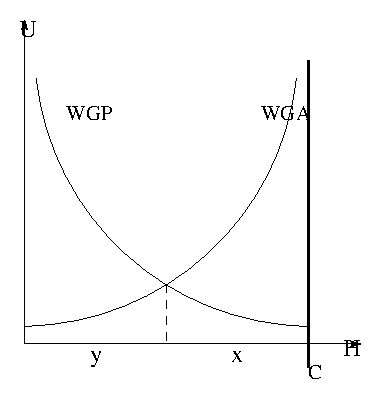
\includegraphics[width=0.49\textwidth]{images/Abbildungen/neuest5.eps}
		\caption{Arbeitsmarkt}
		\hfill \footnotesize\sffamily\textbf{Quelle:} eigene Darstellung
		\label{Grenzentlohnung}
		\vspace{0.48cm}
	\end{figure}

Dieser Zusammenhang wird in Abbildung \ref{Grenzentlohnung} dargestellt. Der Schnittpunkt beider Grenzprodukte der Sektoren 1 und 2 zeigt die Verteilung der Arbeitsplätze der gesamten Bevölkerung auf die jeweiligen Sektoren mit dem einheitlichen gleichgewichtigen Lohnsatz. 


\section[Mikroökonomisches Gleichgewicht]{Mikroökonomisches Gleichgewicht\sectionmark{mikroökonom. GG}}\label{sec:mikro GG}
\sectionmark{mikroökonom. GG}
Das Grundgerüst des Modells von \citet{Acemoglu.2006} wurde auch auf der mikroökonomischen Ebene übernommen. Es unterscheiden sich auch hier Manager hinsichtlich ihres Alters und ihrer technischen Qualitäten. Beides bedingt die Projektgrö{\ss}e, die ein Unternehmen durchführen darf. Für den Kapitalisten, der einen Arbeiter als Ingenieur  einstellt, ist letztendlich der resultierende Wert dieser Führungskraft, der durch ihn entstehende zusätzliche Gewinn, von Bedeutung. Bei der Auswahl des technischen Managers muss ein Kapitalist somit alle Kriterien berücksichtigen.\\
Die Qualifikationen, das Alter und die damit verbundene mögliche Projektgrö{\ss}e haben Einfluss auf die Produktivität, die Investitionssumme und letztlich den Gewinn eines Unternehmens. Die folgende Abbildung \ref{fig:technische Eigenschaften} liefert eine Übersicht über die möglichen Eigenschaften und Fähigkeiten eines Ingenieurs mit den entsprechenden Kombinationsmöglichkeiten.\\


	\begin{figure}[H]
		\vspace{0.43cm}
		\centering 
		\begin{tikzpicture}[node distance=1cm, auto]  
			\tikzset{
			mynode/.style={rectangle,rounded corners,draw=black, top color=white, bottom color=green!50,very thick, inner sep=1em, minimum size=3em, text centered},
			myarrow/.style={thick},
			mylabel/.style={text width=5em, text centered}, 
			myline/.style={shorten >=1pt, thick}
			}  
			\node[mynode] (unternehmer) {Ingenieur};  
			\node[below=2cm of unternehmer] (dummy) {}; 
			\node[mynode, left=of dummy] (JUNG) {jung};  
			\node[mynode, right=of dummy] (ALT) {alt};
			\node[mylabel, left=of JUNG] (label1) {Alter};  
			%\node[mylabel, below right=of unternehmer] (label2) {Participation rate $\theta_2$};
			% The text width of 7em forces the text to break into two lines. 
			\node[mynode, below=of JUNG](KLEIN){klein};
			\node[mynode, below=of ALT](GROSS){gro{\ss}};
			\node[mylabel, left=of KLEIN] (label2) {Projektgrö{\ss}e};  
			\node[mynode, below=of KLEIN](UNKNOWN){unbekannt};
			\node[mynode, below right=1.43cm of GROSS](HIGH){hoch};
			\node[mynode, left= of HIGH](LOW){gering};
			\node[mylabel, left=of UNKNOWN] (label3) {Qualifikation};  
			\node[mynode, below=of UNKNOWN](INNOVATIV){?innovativ?};
			\node[mynode, below=of LOW](LIQUIDE){liquide};
			\node[mynode, below=of HIGH](INNOQUIDE){\parbox{1.8cm}{innovativ\\ + liquide}};
			\node[mylabel, left=of INNOVATIV] (label4) {Potenzial};			
			\draw[myarrow] (unternehmer.south)  ++(0,0) -- ++(0,-1) -|  (JUNG.north);	
			\draw[myarrow] (unternehmer.south)  ++(0,0) -- ++(0,-1) -|  (ALT.north);
			\draw[myline] (JUNG.south) ++(0,0) -- ++(0,-1) -|  (KLEIN.north);	
			\draw[myline] (ALT.south) ++(0,0) -- ++(0,-1) -|  (GROSS.north);	
			\draw[myline] (KLEIN.south) ++(0,0) -- ++(0,-1) -|  (UNKNOWN.north);
			\draw[myarrow] (GROSS.south) -- ++ (0,0) -- ++(0,-.6) -|  (LOW.north);	
			\draw[myarrow] (GROSS.south) -- ++ (0,0) -- ++(0,-.6) -|  (HIGH.north);
			\draw[myline] (UNKNOWN.south) -- ++(0,0) -- ++(0,-1) -|  (INNOVATIV.north);
			\draw[myline] (LOW.south) -- ++(0,0) -- ++(0,-1) -|  (LIQUIDE.north);
			\draw[myline] (HIGH.south) -- ++(0,0) -- ++(0,-1) -|  (INNOQUIDE.north);
			%\draw[<->, >=latex', shorten >=2pt, shorten <=2pt, bend right=45, thick, dashed] 
			(JUNG.south) to node[auto, swap] {Competition}(ALT.south); 
			% The swap command corrects the placement of the text.
		\end{tikzpicture}\\
		%\medskip
		\hfill \footnotesize\sffamily\textbf{Quelle:} eigene Darstellung
		\caption{Eigenschaften eines Ingenieurs} 
		\label{fig:technische Eigenschaften}
	\end{figure}


Als Ingenieure angestellte Arbeiter werden als gut ausgebildete Personen mit ausgeprägten technischen Fähigkeiten kategorisiert, wenn $\gamma_t >1$ gilt. Weisen Arbeiter einen geringeren Bildungsstand auf, so sind sie mit weniger qualifizierenden technischen Fähigkeiten ausgestattet, sodass  $\gamma_t=0$ gilt. Bezüglich des qualitativen Bildungsstandes wird demzufolge zwischen hoher Qualifizierung der technischen Geschäftsführung durch eine modernere Bildung und eher traditionell und dann relativ weniger gut ausgebildeten technischen Managern bzw. Ingenieuren unterschieden.\\
Werden die Arbeiter neu eingestellt, so ist den Unternehmungen noch nicht bekannt, mit welchen Fähigkeiten die zukünftigen Ingenieur  ausgestattet sind. In diesem Fall handelt es sich um junge technische Geschäftsführer, die noch keine nennenswerte Berufserfahrung aufweisen können.\\ 
Die Wahrscheinlichkeit, dass der eingestellte Ingenieur mit hohen Fähigkeiten ausgestattet ist, beträgt $\lambda$ und mit einer Wahrscheinlichkeit von $(1-\lambda)$ ist die Ausbildung des Ingenieurs von geringer Qualität.\\
Weiterhin werden die Ingenieure neben ihren unternehmerischen und technischen Qualitäten auch anhand des Alters unterschieden. Haben die technischen Manager bereits eine Periode gearbeitet, werden sie als "`alt"' klassifiziert. Aufgrund der vorhandenen Erfahrung und der gemeinsamen Zusammenarbeit sind dadurch dem Unternehmen die Fähigkeiten der Angestellten bekannt.\\
Kategorisiert nach ihren Eigenschaften, sind die Ingenieure in zwei verschiedenen Unternehmensbereichen dienlich und bedingen damit die Strategie, denn es liegt an den Kenntnissen und Fähigkeiten der Ingenieure, ob ein Unternehmen sich auf die Imitation oder Innovation konzentriert. Innovationen können die Produktivität erhöhen und den Gewinn eines Unternehmens steigern, wozu qualifizierte Ingenieure notwendig sind. Ältere Ingenieure können hingegen die Kapitalisten durch ihre Einlage auch finanziell unterstützen. Diese Liquidität stellt ebenfalls einen Anreiz für das Unternehmen dar, da dies dem Ingenieur ermöglicht, die Projektgrö{\ss}e mit zu beeinflussen. Bei diesem Entscheidungsproblem entsteht ein Trade-off, der in Kapitel \ref{sec:Strategiewahl} noch relevant und dann genauer betrachtet wird.


\subsection{Finanzierung der Unternehmung}
Die hier aufgeführten Finanzierungsmöglichkeiten der Unternehmen wurden ebenfalls aus dem Modell von \citet{Acemoglu.2006} übernommen.
Die Eigentümer der Unternehmen, die Kapitalisten, benötigen zum einen Geld, um den Ingenieur sowie Arbeiter einzustellen und zum anderen, um die Finanzierung der Projekte zu gewährleisten. Ferner liegt ein unvollkommener Kapitalmarkt vor. \\
Eine monetäre Bezugsquelle ist der Kapitalist selbst. Dieser ist in der Lage, die grundlegenden Kosten zu decken, um kleine Projekte durchzuführen. Dabei handelt es sich nicht um Vermögen, welches von au{\ss}en in die Unternehmung bzw. in das Modell einflie{\ss}t. \\


Neben dem Kapitalisten kann auch der Ingenieur einen Beitrag zur finanziellen Situation des Unternehmens leisten. Die Finanzierungsart hängt wiederum von dem Alter der Unternehmen ab. Eine Neugründung hat eingeschränktere finanzielle Möglichkeiten als ein bereits bestehendes, erprobtes Unternehmen. In neu gegründeten Unternehmen können junge Kapitalisten  mit Hilfe von Darlehen die notwendigen Anfangsinvestitionen tätigen. Die Darlehen werden ihm von seinen Konkurrenten gewährt und stellen keine Markteintrittsbarriere dar. In diesem Fall ist auch der Ingenieur "`jung"' bzw. unerfahren und hat keine liquiden Mittel, die er in das Unternehmen einflie{\ss}en lassen kann.\\
Kapitalisten bestehender "`alter"' Firmen verfügen zusätzlich zu den Darlehen anteilig über die erwirtschafteten Gewinne vorheriger Projekte, die reinvestiert werden.\\
Die Möglichkeit, dass der angestellte Ingenieur die finanzielle Lage der Unternehmung verbessern kann, besteht nur bei bereits vorhandenen und somit etablierten Unternehmen, die ältere Ingenieure beschäftigen. Aus vorangegangenen Projekten erhielten die Ingenieure ein Gehalt mit darin enthaltener Gewinnbeteiligung. Nur mit Hilfe dieser Ersparnis aus der Gewinnbeteiligung können nun auch gro{\ss}e Projekte finanziert werden.\footnote{Die Notwendigkeit der Gewinnbeteiligung wird im folgenden Kapitel \ref{Moral Hazard und Gewinnbeteiligung} diskutiert.}\\


Es ist nur den Kapitalisten vorbehalten, Darlehen aufzunehmen. Die Ingenieure unterliegen Kreditbeschränkungen, weswegen die grö{\ss}ere Last der Investitionskosten durch den Kapitalisten getragen werden muss, obwohl dieser nur einen Anteil von $(1-\mu)$  der Gewinne erhält. 

\subsubsection{Moral Hazard und Gewinnbeteiligung}\label{Moral Hazard und Gewinnbeteiligung}


Als Folge des unvollkommenen Kapitalmarktes und indirekter Folgen des Moral Hazards können Unterinvestitionen durchgeführt werden. Es kann vorkommen, dass Unternehmen sich für kleinere Projekte entscheiden, obwohl höhere Investitionen aus sozialer Sicht effizienter wären. Gerade bei neu gegründeten Unternehmen muss der Kapitalist die vollen Investitionskosten allein tragen. In diesem Fall kommt es besonders häufig zu Unterinvestitionen, weil er nicht bereit ist, das gesamte Risiko für gro{\ss}e Projekte ohne die finanzielle Beteiligung der Mitarbeiter zu tragen.\\


In beiden Fällen können die Investitionsmöglichkeiten älterer Ingenieure das Problem mindern. Die angesprochene Gewinnbeteiligung resultiert in diesem Modell aus dem Umgang mit Moral Hazard. Es kommt zum Problem des Moral Hazards, wenn ein Wirtschaftssubjekt (Agent) besser über die eigenen Handlungen informiert ist, als das andere Individuum (Prinzipal), in dessen Auftrag diese Aufgaben und Pflichten erfüllt werden sollten. In diesem Fall ist es dem Kapitalisten, dem Prinzipal, nicht möglich die operativen und auch innovativen Anstrengungen des Ingenieurs, des Agenten,  zu bewerten und dessen vollen Arbeitseinsatz zu beurteilen. Diese Informationsasymmetrie führt zu dem Problem verzerrter Anreize. Der Agent erfüllt seine Verpflichtung mit möglicherweise minimalem Arbeitseinsatz, wohingegen dann dem Prinzipal aufgrund des Mangels an Sorgfalt unnötige Kosten entstehen. Da der Kapitalist die Arbeitsabläufe weder überwachen noch hinsichtlich sorgfältiger Ausführung kontrollieren kann, wird davon ausgegangen, dass der Agent anteilig Kosten $\mu$ verursacht.\footnote{Zu einem späteren Zeitpunkt wird ersichtlich, dass dieser Aufwand der Gewinnbeteiligung des Ingenieurs entsprechen muss.} Bei diesen Kosten kann es sich auch um veruntreute Gelder handeln, die für private Zwecke genutzt werden. Der Agent hat einen Anreiz, seinen eigenen Nutzen zu maximieren und fügt dabei dem Unternehmen einen finanziellen Schaden zu, der durch die Höhe von $\mu$ gemessen werden kann. Er zeigt auch gleichzeitig den Grad der Unvollkommenheit des Kapitalmarktes, die durch dieses Anreizproblem entsteht.\\ 


Gemindert werden kann dieses Problem aber nicht nur durch Mechanismen der Überwachung und Kontrolle, sondern auch durch eine neue Ausrichtung der Anreize. Der Agent muss die Auswirkungen des Problems selbst mit erleiden, um im eigenen Interesse sorgfältiger zu handeln. Dies kann durch eine Selbstbeteiligung wie bei Versicherungen oder in einem Unternehmen durch Gewinn- oder Umsatzbeteiligung gewährleistet werden. Dadurch ist der Agent motivierter, seine Aufgabe gründlicher und gewissenhafter zu erledigen, weil entstehende Kosten ihn nun selbst betreffen.\footnote{Beispiel Moral Hazard: Die Finanzkrise aus dem Jahr 2008 zeigt beispielhaft die möglichen Auswirkungen des Problems. Dabei führte der Moral Hazard zu einer Mentalität höherer Risikobereitschaft im amerikanischen Finanzsystem. Das Problem des Moral Hazard lag in den angedachten Bonuszahlungen für Bankenmanager. Sie versuchten, ihre jährliche Gewinnbeteiligung auszudehnen, indem risikoreiche Investitionen getätigt wurden, die einen deutlich höheren Gewinn versprachen. Da der Bankenmarkt immer mit staatlicher Unterstützung rechnen konnte, rechneten die Manager nicht mit weitreichenden Konsequenzen im Falle einer Fehlinvestition.}\\
%Text {Krugman 2010 #75S: 583–584} Fu{\ss}note:{Mankiw 2012 #76S: 574–575}
Für den Umgang mit diesem Problem haben auch \citet{Acemoglu.2006} im Rahmen dieses Modells eine Gewinnbeteiligung eingeführt. Den Agenten (Ingenieuren) steht nach einer Periode ein Anteil des Gewinns $\pi_t(\nu|s,e,z)$ zu.\\
Dabei beschreibt $s$ die Projektgrö{\ss}e, $e$ das Alter des Ingenieurs und $z$ die Qualifikationen dessen.\footnote{Die Parameter werden im folgenden Kapitel \ref{sec:Strategiewahl} noch einmal genauer erläutert und definiert.}  Aus der Gleichung  \eqref{Gewinn Zwischengutsektor} zusammen mit Gleichung \eqref{Produktivitat} ergibt sich:

	
	\begin{equation}
		\pi_t(\nu)=\delta s_t(\nu)[\eta\overline{A}_{t-1}+\gamma_t(\nu)A_{t-1}]N_t
	\end{equation}


Diese Gleichung bildet die direkte Abhängigkeit des Gewinns zu den Eigenschaften des Ingenieurs (Projektgrö{\ss}e, Alter und Ausbildung) ab.  Damit das Problem des Moral Hazards gemindert wird und die Unternehmer keine Erträge an sich nehmen, die ihnen nicht zustehen, muss deren Gehalt $W_t(\nu|s,e,z)$ grö{\ss}er sein als der Gewinnanteil $\mu\pi(\nu|s,e,z)$, der möglicherweise entwendet werden kann und es gilt demnach:


	\begin{equation}
		W_t(\nu|s,e,z)-\mu\pi(\nu|s,e,z)\geq 0
	\end{equation}


Diese Restriktion führt auch dazu, dass eine vertragliche Regelung, die eine Weiterbeschäftigung nur bei sorgfältiger und vollständiger Erfüllung der Aufgaben vorsieht, hinfällig wird. Denn wird der Ingenieur zusätzlich durch eine Gewinnbeteiligung vergütet, dann stellt dies einen Anreiz dar, jegliche Aufgaben und Pflichten gewissenhaft zu erledigen, um weiterhin im Unternehmen als Ingenieur angestellt zu bleiben. Der Ingenieur ist zudem motiviert, den Jahresumsatz und damit möglichst auch den Gewinn langfristig zu steigern, um seine persönliche Bonuszahlung zu erhöhen.\\


Die Gestaltung dieses Modells wird dadurch auf zwei Weisen beeinflusst. Moral Hazard führt hier zu Kreditbeschränkungen und schränkt damit das Investitionsvolumen vor allem junger Ingenieur ein, die keine Gewinnbeteiligung aus vorherigen Projekten haben. Sie können keine Sicherheiten vorweisen und ihre Liquidität ist geringer als die der älteren Ingenieure. Es können keine gro{\ss}en Projekte durchgeführt werden, die eine hohe Investitionssumme erfordern, weil ein junger Ingenieur nicht in Vorlage gehen kann.\\
Dies ist für die älteren, weniger qualifizierten Ingenieure von Vorteil und erhöht deren Wert für ein Unternehmen. Au{\ss}erdem schützen diese anteiligen Gewinnausschüttungen die traditionell ausgebildeten älteren Ingenieure davor, durch junge Ingenieure ersetzt zu werden. Die finanziellen Mittel steigern die Attraktivität und ermöglichen einen ausgeglicheneren indirekten Wettbewerb mit den möglichen hohen unternehmerischen und letztlich innovativen Fähigkeiten der jungen Ingenieure. Die Gewinnbeteiligung hat also in doppelter Art einen positiven Effekt auf das Unternehmen. Zum einen mindern sie die Veruntreuung von Geldern und zum andern können diese Mittel von den älteren Ingenieuren reinvestiert werden. Dadurch werden dem Unternehmen in einer zukünftigen Periode zusätzliche finanzielle Mittel zur Verfügung gestellt, um gro{\ss}e Projekte bearbeiten zu können. \\


Der ausgeschüttete Gewinn ist begrenzt durch die Kosten einer Investition, $\widehat{RE}_t(\nu|s,e,z)\leq k_t(\nu|s)$. Au{\ss}erdem unterliegen sie noch einer weiteren Restriktion:


	\begin{equation}
		0\leq\widehat{RE}_t(\nu|s,e,z)\leq RE_t(\nu|s,e,z)
	\end{equation}

Die gesamten Gewinnrücklagen eines Unternehmens $RE_t(\nu|s,e,z)$ müssen mindestens der Gewinnbeteiligung des Managers entsprechen. Dies verhindert beispielsweise zusätzliche Zahlungen des Ingenieurs an den Kapitalisten, was zu ungenauen Machtverhältnissen führen kann. \\


Letztlich führt die Minderung des Moral Hazard Problems durch die Einführung von Gewinnbeteiligungen zu einem Trade-off zwischen jungen, finanzschwachen und älteren, finanzstarken Ingenieuren. 


\subsection{Strategiewahl}\label{sec:Strategiewahl}
Das angedeutete Entscheidungsproblem ist Kern des mikroökonomischen Gleichgewichts und wird im Folgenden genauer erläutert. Die strategischen Hauptentscheidungen dieses Modells werden durch den Kapitalisten einer Unternehmung getroffen. Dabei spielen die Eigenschaften der angestellten Ingenieure und die damit verbundene Projektgrö{\ss}e eine wichtige Rolle. \\
Die unternehmerische Tätigkeit eines Angestellten gliedert sich in diesem Modell in zwei Aufgabenfelder. Zum einen sollen neue Technologien erfunden werden, wozu die Fähigkeiten und Qualifikationen wichtig sind. Zum anderen sollen bereits vorhandene Technologien der WTG nachgeahmt werden, wofür grundsätzlich keine speziellen Fachkenntnisse benötigt werden, wie es bei der Innovationsentwicklung erforderlich ist. 


\subsubsection{Imitative Tätigkeit}
Für die Imitation bereits bekannter Produktionstechniken oder Güter bedient sich ein Unternehmen dem Wissensstand der WTG und ahmt mit Hilfe dieser die Produkte oder Produktionsprozesse nach. Der Illustration dient wieder das Beispiel der Textilindustrie. Durch den Erwerb von Gütern der Konkurrenten können diese hinsichtlich ihrer Herstellungsprozesse studiert werden. Dabei kann festgestellt werden, dass beispielsweise eine neue stabilere Naht das Endprodukt verbessert und zu effizienteren Arbeitsabläufen führt. Hierfür ist die Qualität der Ausbildung der Ingenieure nicht so sehr von Bedeutung. Adaptive Tätigkeiten fordern lediglich eine genaue Beobachtungsgabe und die Beherrschung traditioneller Arbeitsweisen. In diesem Beispiel zählen der Umgang mit einer Nähmaschine und das Anfertigen von Schnittmustern zu diesen Grundfertigkeiten.


\subsubsection{Innovative Tätigkeit} 
%\textit{Innovative Tätigkeit}\\
Für die Erfindung neuer Prozesse ist es jedoch sehr wichtig, dass es sich um hoch qualifizierte Ingenieure handelt, da hier vor allem selbstständiges und vorausschauendes Denken vorausgesetzt wird. Die Entwicklung der angesprochenen Naht fordert neben den allgemeinen Grundkenntnissen auch Kenntnisse über die Beschaffenheit der Materialien wie Stoff, Faden und Nähmaschine sowie darüber hinaus noch die Fähigkeit, die Wirkung neuer Kombinationsmöglichkeiten zu erfassen. Ziel der innovativen unternehmerischen Tätigkeiten ist das Erkennen vorhandener Probleme und eine daraus folgende Problemlösung. 


\subsubsection{Entscheidungsprozess}
Wenn sich der Kapitalist dazu entscheidet junge Ingenieure einzustellen, so ist es unvorhersehbar, welche Qualifikationen diese mit sich bringen. Sind die Fähigkeiten eines Ingenieurs bekannt, kann über dessen Entlassung oder dessen Verbleib im Unternehmen entschieden werden. Für ältere, hoch qualifizierte Ingenieure besteht ein Nachfrageüberschuss, sie werden nicht mehr aus einem Unternehmen entlassen. Denn gerade das benötigte Know How und somit das Potenzial, technischen Fortschritt zu generieren, ist sehr profitabel und beliebt. Es ist zu entscheiden, ob ein erfahrener Ingenieur mit geringer Qualifikation in dem Unternehmen bleiben soll oder nicht. Der Entscheidungsfindung dient eine genaue Analyse beider Alternativen, anhand der Abschätzung der resultierenden Wertigkeiten der Ingenieure für das jeweilige  Unternehmen.\\
Zunächst wird der Wert jeder Alternative einzeln betrachtet. Dabei gilt in diesem Modell, dass ein Ingenieur entweder jung oder alt ist mit $e\in\left\{Y,O\right\}$. Die Qualifikation bemisst sich an der Art der Ausbildung, die gut bzw. modern sein kann oder eher schlecht damit traditionell geprägt ist, mit $z\in\left\{L,H\right\}$. Au{\ss}erdem hängt der Wert einer Alternative von der Projektgrö{\ss}e ab, die gro{\ss} oder klein sein kann, $s\in\left\{\sigma_j,1\right\}$.


	\begin{equation}
		V_{tj} (\nu|s=1,e=O,z=L)=[(1-\mu)\delta_j N_j \eta\overline{A}_{t-1}-max(\kappa\overline{A}_{t-1}-RE_t,0)]\label{Wert}
	\end{equation}


Gleichung \eqref{Wert} gibt den Wert älterer, traditionell ausgebildeter Ingenieur an, die gro{\ss}e Projekte bearbeiten. Dieser setzt sich zusammen aus dem erwirtschafteten Gewinn durch imitative Tätigkeiten $\delta_j N_j \eta\overline{A}_{t-1}$, abzüglich dem ausgeschütteten Gewinn an die Ingenieure $\mu\delta_j N_j \eta\overline{A}_{t-1}$ und der maximalen Kosten $\kappa\overline{A}_{t-1}-RE_t$. Dabei wird im Folgenden davon ausgegangen, dass die Kosten des Projekts die eingebrachten Gewinne $RE_t$ überschreiten, $\kappa\overline{A}_{t-1}>RE_t$. Diese älteren Ingenieure sind grö{\ss}tenteils für nachahmende Prozesse geeignet und scheinen zunächst weniger attraktiv. Doch durch das Einbringen ihrer gesparten Gewinnanteile steigern sie ihren Marktwert. Denn der unvollkommene Kapitalmarkt führt bei den Unternehmen, zu grö{\ss}eren Investitionen und damit wird die Durchführung gro{\ss}er Projekte ermöglicht. Die Vorzüge grö{\ss}erer Projekte liegen in höheren erwarteten Gewinnen, jedoch ist auch mit höheren Kosten zu rechnen. Grö{\ss}ere Projekte führen gemä{\ss} \eqref{Produktivitat} zu einer höheren Produktivität, weil Unterinvestitionen vermieden werden und dadurch die Effizienz gefördert wird, obwohl weniger qualifizierte Ingenieure nicht innovativ tätig sind. 


	\begin{equation}
		E_tV_{tj} (\nu|s=\sigma_j,e=y)=(1-\mu)\delta_j N_j\sigma_j(\eta +\lambda\gamma a_{j t-1})\overline{A}_{t-1}-\phi\kappa\overline{A}_{t-1}\label{erwarteter Wert}
	\end{equation}

Gleichung \eqref{erwarteter Wert} ist die formale Darstellung des erwarteten Marktwertes junger Ingenieure und setzt sich wie folgt zusammen: 
Von dem jeweiligen möglichen Gewinn aus Imitation $\eta\delta_j N_j\sigma_jv$ bzw. Innovation $\lambda\gamma a_{j t-1}\delta_j N_j\sigma_j$ werden jeweils die Gewinnbeteiligungen der Ingenieure $-\mu\delta_j N_j\sigma_j(\eta +\lambda\gamma a_{j t-1})$ subtrahiert. Von diesem Ertrag werden noch die Kosten in Höhe von $\phi\kappa\overline{A}_{t-1}$ abgezogen. 

Die Untersuchung junger Ingenieure deren Fähigkeiten noch unbekannt sind, zeigt, dass der Kapitalist die Finanzierung der Projekte allein realisieren muss. Das Unternehmen kann keine ersparten Gewinnbeteiligungen dieser Mitarbeiter beziehen, weil es sich um relativ junge und somit unerfahrene Ingenieure handelt. \\
Mit einer Wahrscheinlichkeit von $(1-\lambda)$ handelt es sich um einen weniger qualifizierten Manager. Stellt sich jedoch heraus, dass der junge Ingenieur hohe Qualifikationen mit sich bringt, könnte der Aspekt der fehlenden Ersparnis durch innovative Tätigkeiten ausgeglichen werden. Ein höherer Bildungsstand und damit verbundener technischer Fortschritt nutzt der Unternehmung ebenso wie die Durchführung gro{\ss}er Projekte. Durch Innovationen steigt in der Regel auch die Absatzmenge an, selbst wenn insgesamt das Verkaufsvolumen kleinerer Projekte geringer ist. \\
Nachdem beide Möglichkeiten analysiert wurden, muss das Unternehmen abwägen, ob es einen alten, erfahrenen Ingenieure mit traditioneller Ausbildung behalten möchte oder diesen durch einen jungen Ingenieur ersetzt. Es stellt sich also die Frage, ob die Investitionen älterer Ingenieure attraktiver sind als die möglichen innovativen Fähigkeiten eines neuen Ingenieurs. Damit sich ein Unternehmen gegen die Entlassung erfahrener, traditionell ausgebildeter Ingenieure entscheidet, muss  Ungleichung \eqref{Wertvergleich} gelten, in der die Wertigkeit beider Alternativen gegeneinander abgewogen wird.


	\begin{equation}
		V_{tj}(\nu|s=1,e=o,z=L) > E_t V_{tj} (\nu|s=\sigma_j,e=y)\label{Wertvergleich}
	\end{equation}


Der Wert eines älteren, schlecht ausgebildeten Ingenieurs, mit dessen Hilfe gro{\ss}e Projekte finanziert werden können, muss höher sein als der erwartete Marktwert, wenn das Unternehmen einen jungen Ingenieur einsetzt, mit dem kleine Projekte realisiert werden und dessen Fähigkeiten noch unbekannt sind. Ist dies nicht der Fall, wird der Ingenieur entlassen und ein junger Mitarbeiter wird neu eingestellt, weil es für das Unternehmen nicht mehr lohnend ist, den älteren Ingenieur weiter zu beschäftigen. \\
Die eingebrachten Gewinnbeteiligungen der Ingenieure müssen die höheren Kosten grö{\ss}erer Projekte kompensieren können und sogar höher sein, als die Gewinne, die in kleinen, möglicherweise innovativ ausgerichteten Projekten realisiert werden, damit das Arbeitsverhältnis bestehen bleibt. \\
Bei dieser Personalentscheidung werden die erfahrenen, hoch qualifizierten Mitarbeiter nicht berücksichtigt, da diese am "`beliebtesten"' sind und die Unternehmensstruktur mit innovativen Tätigkeiten prägen sowie zur Finanzierung gro{\ss}er Projekte beitragen.\\
Diese Rangfolge spiegelt sich auch in der Gehaltsstruktur wieder. Die Entlohnung der älteren, hoch qualifizierten Ingenieure ist höher, als die der älteren, weniger gut ausgebildeten und letztlich erzielen die jungen Ingenieure das geringste Einkommen.



\section[Makroökonomisches Gleichgewicht]{Makroökonomisches Gleichgewicht\sectionmark{Makroökonom. GG}}\label{sec:makro GG}
\sectionmark{Makroökonom. GG}
%dann im makro GG, wenn gilt: Volkseinkommen $=$ BIP
Beim makroökonomischen Gleichgewicht werden die mikroökonomischen Entscheidungen der Unternehmen akkumuliert. Dies bedingt die durchschnittliche Produktivität eines Landes und die daraus resultierende Lage zur WTG. Folglich ist die LTG äquivalent mit der Produktivität des führenden Unternehmens eines Zwischengutsektors, $A^H \Leftrightarrow A_t(\nu)$.\\
Der Abstand zur WTG wird in diesem Kapitel, so wie auch bei \citet{Acemoglu.2006}, mit Hilfe der durchschnittlichen Produktivität \eqref{Produktivitat} eines Landes ermittelt.
Diese ergibt sich aus den Entscheidungsalternativen der Kapitalisten. Im Folgenden werden die möglichen Produktivitäten eines Unternehmens erläutert, abhängig von der bisherigen personellen Besetzung und Strategiewahl. Dabei wird zwischen drei Möglichkeiten unterschieden: 1. die Unternehmen beschäftigen nur junge Ingenieure, 2. sie nehmen keine Personalveränderungen vor oder 3. die Unternehmen nehmen Personalveränderungen vor, indem weniger qualifizierte Ingenieure gegen junge ausgetauscht werden.\\
Im ersten Fall werden die neu gegründeten Unternehmen betrachtet, die nur junge, unerfahrene Ingenieur einstellen können. Die Fähigkeiten der Ingenieure sind ungewiss und mit einer Wahrscheinlichkeit von $\lambda$ relativ hoch und mit einer Wahrscheinlichkeit von $(1-\lambda)$ relativ gering.


	\begin{equation}
		A_{tj}^{y}=\sigma_j(\eta\overline{A}_{t-1}+\lambda\gamma A_{t-1})\label{Produktivitat jung}
	\end{equation}


Die Produktivität der jungen Ingenieure $A_{tj}^{y}$ ist in erster Linie von der Qualifikation der Ingenieure abhängig. Das Wissen der LTG $A_{t-1}$ kann nur durch die qualifizierten, innovativ arbeitenden Ingenieure, $\gamma$, mit einer Wahrscheinlichkeit von $\lambda$ genutzt werden.\footnote{Es werden Innovationen mit einer Wahrscheinlichkeit von $\lambda$ entwickelt. Dem Gesetzt der gro{\ss}en Zahl folgend entspricht $\lambda$ der Anzahl der Sektoren, die erfolgreich innovieren, also der Häufigkeit von Innovationen in einer Periode.} Das lokale technische Wissen der Vorperiode $\overline{A}_{t-1}$ steht allen Ingenieuren der Volkswirtschaft zur Verfügung und dient der Imitation von Gütern und Prozessen. Bei $\eta$ handelt es sich um die Imitationsintensität, die angibt wie stark sich die Technologie verändert hat und wie intensiv die Technologien der WTG eingesetzt wird.\\


Bei der 2. und 3. Entscheidungsmöglichkeit handelt es sich um die Produktivität älterer Unternehmen, die seit mindestens einer Periode Ingenieure angestellt haben und es zu entscheiden gilt, ob die weniger gut ausgebildeten Ingenieure weiterhin angestellt bleiben $A_{tj}^{o}[R_{tj}=0]$ oder durch junge ersetzt werden $A_{tj}^{o}[R_{tj}=1]$. \\


Die Wahl der jeweiligen Alternative wird durch das mikroökonomische Gleichgewicht determiniert. Wird sich für die Weiterbeschäftigung aller Ingenieure eingesetzt, besteht die Ingenieurstruktur aus Ingenieuren beider Bildungsschichten. Die Erfahrung aller und die finanzielle Unterstützung der Ingenieure ermöglicht es nur noch gro{\ss}e Projekte durchzuführen mit $s=1$.


	\begin{equation}
		A_{tj}^{o}[R_{tj}=1]=\eta\overline{A}_{t-1}+\lambda\gamma A_{t-1}\label{Produktivitat nur alte}
	\end{equation}


Bei der anderen Alternative werden nur die weniger qualifizierten Ingenieure entlassen. Die hoch qualifizierten verbleiben im Unternehmen und bearbeiten gro{\ss}e Projekte. Wohingegen die nun neu eingestellten jungen Unternehmen mit kleineren Projekten, $s=\sigma_j$, vertraut werden. 


	\begin{equation}
		A_{tj}^o[R_{tj}=0]=\lambda(\eta\overline{A}_{t-1}+\gamma A_{t-1})+(1-\lambda)\sigma_j(\eta\overline{A}_{t-1}+\lambda\gamma A_{t-1})\label{Produktivitat alt und jung}
	\end{equation}


Es wird angenommen, dass es sich bei der Hälfte aller Unternehmen um Neugründungen handelt. Dabei wird die Gesamtheit aller Produktivitäten eines Sektors und somit aller Unternehmen eines Sektors in einem Land betrachtet. 


	\begin{equation}
		A_{tj}\equiv\int_0^1 A_{t}(\nu)d\nu=\frac{(A_{tj}^y+A_{tj}^o)}{2} \label{Produktivitat gesamt}
	\end{equation}


Nachdem nun die Produktivität eines Landes beleuchtet wurde, wird die Wachstumsrate der aggregierten Produktivität $\frac{A_t}{A_{t-1}}$ genauer definiert die sich aus den Gleichungen \eqref{Produktivitat} und \eqref{durchschnittliche Technologie} ergibt.


	\begin{equation}
		\frac{A_t}{A_{t-1}}\equiv\frac{\int_0^1A_{t}(\nu)d\nu}{A_{t-1}}=\int_0^1s_{tj}(\nu)\left[\eta\frac{\overline{A}_{t-1}}{A_{t-1}}+\gamma_t(\nu)\right]d\nu
		\label{WachstumTechnologie}
	\end{equation}


Dieser Term beschreibt die Bedeutung des Abstandes zur WTG für den technologischen Fortschritt, der wiederum definiert ist als: 


	\begin{equation}
		a_{tj}\equiv\frac{A_{tj}}{\overline{A}_{tj}}\label{kleinA}
	\end{equation}


Ist der Quotient $\frac{\overline{A}_{t-1}}{A_{t-1}}$ aus Gleichung \eqref{WachstumTechnologie} relativ hoch, dann wird das technische Wachstum hauptsächlich durch imitative Tätigkeiten generiert, das Land liegt dann relativ weit von der WTG entfernt. Je kleiner der Abstand zur WTG, desto unbedeutender sind nachahmende Prozesse für die Produktivität eines Landes. Die Bedeutung von Innovationen ist dann deutlich höher und die Fähigkeiten des Ingenieurs $\gamma$ beeinflussen den Fortschritt wesentlich.\footnote{Eine abnehmende Annäherung an die WTG wird gewährleistet, wenn $\lambda\gamma<1$ gilt.}
Mit sinkender Distanz zur WTG nimmt die Bedeutung der Innovationsstrategie zu und damit wird auch eine zielgerichtete Wahl geeigneter Ingenieure wichtiger, wodurch sich der Schwerpunkt auf kurzfristige Beschäftigungsbeziehungen verlagert.\\


Für die Berechnung des Abstandes zur WTG \eqref{kleinA} werden die Gleichungen \eqref{Produktivitat jung}-\eqref{Produktivitat gesamt} zusammengefasst und ergeben sich für jeden Sektor folgende technologische Entwicklungsstände.\footnote{Die detaillierte Berechnung ist in Appendix \ref{sec:Abstand WTG} zu finden.}


	\begin{equation}
		a_{tj}=\begin{cases}\frac{1+\sigma_j}{2(1+g)}[\eta+\lambda \gamma a_{t-1j}] \hfill\text{if  } R_{tj}=1 \\
		\frac{1}{2(1+g)}[(\lambda+\sigma_j+(1-\lambda)\sigma_j)\eta+(1+\sigma_j+(1-\lambda)\sigma_j)\lambda\gamma a_{t-1 j}] \quad\hfill\text{if   }R_{tj}=0
		\end{cases}\label{Abstand WTG}
	\end{equation}


Jeweils der erste Summand in den eckigen Klammern steht für die nachahmenden Tätigkeiten. Der Vergleich beider Strategien zeigt, dass Wachstum, welches durch Imitationen bei der Strategie der Haltung weniger qualifizierter Manager resultiert, höher ist als das Wachstum bei der Strategie des Austauschs der Ingenieure.

 
	\begin{equation}
		(1+\sigma_j)\eta>(\lambda+\sigma_j+(1-\lambda)\sigma_j)\eta
	\end{equation}


Der zweite Summand beschreibt das Wachstum, das jeweils durch die Innovatiion hervorgerufen wird. Das Ersetzen älterer, weniger qualifizierter Ingenieure durch junge Ingenieure führt zu einem deutlich höheren Wachstum an technologischem Wissen, als es der Fall ist, wenn die Situation im Unternehmen unverändert bleibt und es keine Neueinstellungen gibt.


	\begin{equation}
		(1+\sigma_j)\lambda \gamma a_{t-1j}<(1+\sigma_j+(1-\lambda)\sigma_j)\lambda\gamma a_{t-1j}\footnote{Dies gilt ausgehend von dem Gleichen technologischen Entwicklungsstand $a_{t-1j}$.}
	\end{equation}


Von nun an wird die eben zuerst genannte Strategie der Unternehmen, welche vorwiegend die nachahmenden Tätigkeiten beinhaltet, als Investitions- oder Imitationsstrategie bezeichnet. Die Unternehmensstruktur ist durch gro{\ss}e Projekte geprägt, deren Finanzierung durch die eingebrachten Gewinnbeteiligungen der älteren, weniger qualifizierten Ingenieure ermöglicht wird. Die damit verbundenen hohen Investitionssummen sind unabhängig von der Entwicklung neuer Prozesse oder Produkte. Die Arbeitsabläufe einer Imitation sind relativ schlichter, unkomplizierter und strukturierter, somit sind hohe Qualifikationen des Ingenieurs von geringerer Bedeutung. Die Situation im Unternehmen bleibt in der zweiten Periode unverändert. Es stehen vor allem langfristige Beziehungen von Unternehmen zu Managern im Vordergrund, um das Investitionsvolumen möglichst hoch zu halten. Nicht nur die Erfahrung aller Angestellten, sondern auch resultierende Skaleneffekte aufgrund grö{\ss}erer Produktionsmengen sind ma{\ss}geblich für die Produktivität dieser Unternehmen.\\


Bei der zweiten Strategie wird der Begriff der Innovationsstrategie analog verwendet. Die gering qualifizierten Ingenieur werden entlassen, da diese höhere Kosten verursachen und durch sie der technologische Fortschritt des Unternehmens gehemmt wird. Der geringere Bildungsstand lässt nur nachahmende Tätigkeiten zu und ist somit nicht im Sinne der Innovationsstrategie. Diese Strategie ist durch kurzfristige Beziehungen geprägt und eine hohe Fluktuation der Ingenieure ist die Regel. Es ist den Kapitalisten wichtig, möglichst viele qualifizierte Ingenieure anzustellen. Dafür sind sie bereit, auf die finanziellen Mittel der traditionell ausgebildeten Ingenieure zu verzichten. Neue Ideen führen zu neuen Produktvarianten. Au{\ss}erdem kann durch Verbesserungsvorschläge die Effizienz der Produktion erhöht werden. Neben Start-up-Unternehmen finden junge Ingenieure nur in Firmen, die der Innovationsstrategie folgen eine Anstellung.

\subsection{Gesamtwirtschaftliche strategische Entscheidung bei exogener WTG im technologisch kleinen Land}

Nachdem beide Strategien vorgestellt wurden, hat jedes Unternehmen die Wahl sich für eine der beiden zu entscheiden. In einem technologisch kleinen Land haben Mikroinnovationen keinen Einfluss auf die WTG, die somit exogen gegeben ist. Demzufolge unterscheidet sich auch der mögliche Entwicklungspfad eines technologisch kleinen Landes von einem technologisch gro{\ss}en Land, das Makroinnovationen herstellen kann. Abbildung \ref{fig:ein Sektor exogene WTG} stellt die Abhängigkeit der heutigen technologischen Entwicklungssituation $a_t$ vom gestrigen Entwicklungsstand $a_{t-1}$ dar. Beide Strategien aus Gleichung \eqref{Abstand WTG} sind hier wiederzufinden.\newline


		\begin{figure}[H] 
			\vspace{0.13cm}
			\centering 
			\psfrag{a}{$a$}
			\psfrag{t}{  $_t$}
			\psfrag{-}{  $_-$}
			\psfrag{1}{\, $_1$}
			\psfrag{0.0}[c]{\scriptsize{0}}
			\psfrag{0.2}[c]{\scriptsize{0.2}}
			\psfrag{0.4}[c]{\scriptsize{0.4}}
			\psfrag{0.6}[c]{\scriptsize{}}
			\psfrag{0.8}[c]{}
			\psfrag{1.0}[c]{\scriptsize{1}}
			\begin{overpic}[width=0.9\textwidth]{images/Abbildungen/einSektorExo.eps}
				\put(10.5,0.5){\textcolor{black}{$a_r$}}
				\put(74.5,0.2){\textcolor{black}{$\hat{a}_t$}}
				\put(57.8,-1){\color[rgb]{0.74,0.97,0.22}{$\tilde{a}_{R=1}$}}
				\put(60.1,0.5){\color[rgb]{0,0.32,0}{$\tilde{a}_{R=0}$}}
				%\put(-0.4,12.5){\textcolor{black}{\scriptsize{0.2}}}
				\put(-0.4,34.5){\textcolor{black}{\scriptsize{0.6}}}
				\put(-0.4,45.5){\textcolor{black}{\scriptsize{0.8}}}
				\put(12.8,19.3){\color[rgb]{0,0.32,0}{\textcolor[rgb]{0.74,0.97,0.22}{Innovations-}}}
				\put(12.8,17.1){\color[rgb]{0,0.32,0}{\textcolor[rgb]{0.74,0.97,0.22}{strategie}}}
				\put(5,30){\color[rgb]{0,0.32,0}{\textcolor[rgb]{0,0.32,0}{Imitationsstrategie}}}
			\end{overpic}\\
			\hfill\footnotesize\sffamily{\textbf{Quelle:}}  eigene Darstellung
			\caption{ein Sektor bei exogener Welttechnologiegrenze}
			\label{fig:ein Sektor exogene WTG}
		\end{figure}
		
		
Die Situation ist nur für einen Sektor dargestellt. Die Firmen haben die Wahl zwischen der Imitations- und Innovationsstrategie. Jede Strategie ist durch eine Gerade abgebildet. Diese zeigt die technologische Entwicklung des Sektors bei entsprechender Strategie. Je nach technologischem Entwicklungsstand ist die eine oder die andere Strategie geeigneter, führt also zu einem höheren zukünftigen Entwicklungsstand.\\ 
Der folgende Abschnitt beschreibt drei mögliche Grenzwerte von $a_{t-1}$: $\hat{a}_t$, $a_r$ und $\tilde{a}$.  Bei $\hat{a}_t$ handelt es sich um den Schnittpunkt beider Strategien: Dies zeigt also, ab welchem Entwicklungsstand die Innovationsstrategie zukünftig zu einer höheren Produktivität führt.
Mit dem Überschreiten von $\hat{a}_t$ ist das technologische Wachstum durch die \textcolor[rgb]{0.74,0.97,0.22}{Innovationsstrategie} höher, als durch die bis dahin sinnvollere \textcolor[rgb]{0,0.32,0}{Imitationsstrategie}. 
Für Länder mit einem technologischen Entwicklungsstand, der also grö{\ss}er ist als $\hat{a}_t$, reduziert sich der Abstand zur WTG durch Innovationen schneller, als dies mit der \textcolor[rgb]{0,0.32,0}{Imitationsstrategie} der Fall wäre.\\
Ist der Entwicklungsstand eines Landes höher als der Schwellenwert, dann ist der entgangene zusätzliche Gewinn, hier die Produktivität, durch die relativ schlecht ausgebildeten Ingenieure, die im Unternehmen gehalten werden, zu hoch. Trotz der eingebrachten Gewinnbeteiligung sind junge Ingenieure dem Unternehmen mehr wert. Ist ein Land jedoch noch relativ wenig weit entwickelt und der Abstand zur WTG ist kleiner als $\hat{a}_t$, so ist die \textcolor[rgb]{0,0.32,0}{Imitationsstrategie} ratsam.\\
Nach der Produktivität stehen bei dem zweiten Grenzwert $a_r$ die Gewinne der Unternehmen im Vordergrund. Dieser Schwellenwert wird unter Berücksichtigung der verursachten Kosten der angestellten Ingenieure hergeleitet.\footnote{Die formale Herleitung ist in Appendix \ref{SchwellenwertAr} aufgeführt.}


	\begin{equation}
		a_r{_j}(\mu,\delta)=\frac{[(1-\mu)(1-\sigma_j)+\frac{1+r}{1+g}\mu\sigma_j]\eta-\frac{\kappa(1-\phi)}{\delta N_j}}{(1-\nu)\sigma_j\lambda\gamma} \label{Schwellenwert Kosten}
	\end{equation}


Der Wert $a_r$ gibt an, ab wann es profitabler ist, die Beziehung zu weniger qualifizierten Mitarbeitern zu beenden. Wird dieser überschritten, sind die älteren, weniger qualifizierten Ingenieure trotz der eingebrachten Gewinnbeteiligung zu teuer und es ist lohnender, junge unerfahrene Ingenieure einzustellen. Auch bei diesem Schwellenwert geht es um den Zeitpunkt des Strategiewechsels, jedoch aus einer anderen Perspektive.\\
Die beschriebene und dargestellte Situation entspricht der eines technologisch kleinen Landes bei einer exogenen WTG. Das Unternehmen, welches die Technologie der WTG bereitstellt, arbeitet mit grö{\ss}eren Projekten als das betrachtete Land. Demnach ist es mit kleineren Projekten nicht möglich, dieses Land einzuholen und die WTG zu erreichen.\\ Ein weiterer Grenzwert hinsichtlich des Entwicklungsstandes ist die Nicht-Konvergenz-Falle $\tilde{a}$. In weniger weit entwickelten, technologisch kleinen Ländern führen sehr kleine Projektgrö{\ss}en sowohl mit der Innovations- als auch mit der Imitationsstrategie zu einem technischen Wissenszuwachs. Langfristig konvergieren diese Länder jedoch bis zu einem maximal erzielbaren Wissensstand $\tilde{a}$, der unabhängig von der WTG ist. Anders ausgedrückt können diese Länder nicht zur WTG konvergieren, hier handelt es sich demnach um eine Nicht-Konvergenz-Falle. 
Die Erklärung der Situation für Länder, die mit einem Abstand zur WTG $a_{t-1}>\tilde{a}$ starten, ist etwas komplexer bzw. diffiziler. Zum einen ist fraglich, wie diese technologisch kleinen Volkswirtschaften diesen relativ hohen technologischen Entwicklungsstand erreicht haben. Handelt es sich um Länder in einer Krisensituation, ist es durchaus denkbar, dass sich durch die Verschlechterung der allgemeinen Situation auch die hier angesprochenen Investitionen mindern und dies zu einem Rückgang des technischen Wissens führen könnte. Dann wäre es ihnen kaum noch möglich, Bildungs- und Forschungseinrichtungen aufrecht zu erhalten und es würde  langfristig an der finanziellen Umsetzung von Innovationen und Imitationen scheitern, so dass auch diese Länder in der Nicht-Kovergenz-Falle $\tilde{a}$ münden. Zum anderen könnte es sich auch um Länder handeln, die sehr wahrscheinlich das Wachstum der WTG beeinflussen und hier als obsolet gelten.\\
Je nachdem welche Strategie verfolgt wird, ist einer der beiden folgenden Grenzwerte für $\tilde{a}$ ma{\ss}geblich.\footnote{Die formale Herleitung ist in Appendix \ref{NichtKonvergenzFalleImitation} und \ref{NichtKonvergenzFalleInnovation} zu finden.}


	\begin{equation}
		\tilde{a}_{R=1}=\frac{(1+\sigma_j)\eta}{2(1+g)-\lambda\gamma(1+\sigma_j)}\label{eq:aTilde1}
	\end{equation}


	\begin{equation}
		\tilde{a}_{R=0} = \frac{(\lambda+\sigma+(1-\lambda)\sigma)\eta}{2(1+g)-(1+\sigma+(1-\lambda)\sigma)\lambda\gamma}\label{eq:aTilde0}
	\end{equation}


Die Nicht-Konvergenz-Falle, oder der maximal mögliche Wissensstand $\tilde{a}$ ist in Abbildung \ref{fig:ein Sektor exogene WTG} bei der Innovationsstrategie höher als bei der Imitationsstrategie. Dadurch, dass $a_r<\tilde{a}$ gilt, ist es zwar wirtschaftlicher für die Volkswirtschaft der Innovationsstrategie zu folgen, führt jedoch zu einem geringeren maximal erzielbaren Entwicklungsstand $\tilde{a}_{R=1}$. Durch die Innovationsstrategie kann zwar durch Monopolmacht ein höherer Gewinn erzielt werden, jedoch führt diese zwischen $a_r$ und $\hat{a}_t$ zu einer geringeren Produktivität hinsichtlich des technologischen Fortschritts. Diese geringere Produktivität begründet auch warum ein geringerer technologischer Wissensstand erreicht wird, als mit der Imitationsstrategie. 

Wie aus den Gleichungen \ref{eq:aTilde1} und \ref{eq:aTilde0} ersichtlich ist, variiert die Nicht-Konvergenzfalle mit der Projektgrö{\ss}e.
\newpage
\subsection{Gesamtwirtschaftliche strategische Entscheidung bei endogener WTG im technologisch gro{\ss}en Land}
In technologisch gro{\ss}en Ländern handelt es sich um eine endogene WTG, dann verändert jede Innovation die WTG. Diese Situation ist in Abbildung \ref{fig:ein Sektor endogene WTG} dargestellt.


		\begin{figure}[htb]
			\vspace{0.13cm} 
			\centering 
			\psfrag{a}{$a$}
			\psfrag{t}{  $_t$}
			\psfrag{-}{  $_-$}
			\psfrag{1}{\, $_1$}
			\psfrag{0.0}[c]{\scriptsize{0}}
			\psfrag{0.2}[c]{\scriptsize{0.2}}
			\psfrag{0.4}[c]{\scriptsize{0.4}}
			\psfrag{0.6}[c]{\scriptsize{0.6}}
			\psfrag{0.8}[c]{\scriptsize{}}
			\psfrag{1.0}[c]{\scriptsize{}}
			\begin{overpic}[width=0.9\textwidth]{images/Abbildungen/einSektorEndo.eps}
				\put(23.6,0.4){\textcolor{black}{$a_r$}}
				\put(72.2,-0.1){\textcolor{black}{$\hat{a}_t$}}
				\put(90,0.3){\color[rgb]{0.74,0.97,0.22}{$\tilde{a}_{R=1}$}}
				\put(87,-1.2){\color[rgb]{0,0.32,0}{$\tilde{a}_{R=0}$}}
				%\put(-0.4,12.5){\textcolor{black}{\scriptsize{0.2}}}
				%\put(-0.4,34.5){\textcolor{black}{\scriptsize{0.6}}}
				\put(-0.4,45.5){\textcolor{black}{\scriptsize{0.8}}}
				\put(1,56){\textcolor{black}{\scriptsize{1}}}
				\put(5,20){\color[rgb]{0,0.32,0}{\textcolor[rgb]{0.74,0.97,0.22}{Innovations-}}}
				\put(5,17.8){\color[rgb]{0,0.32,0}{\textcolor[rgb]{0.74,0.97,0.22}{strategie}}}
				\put(5,36){\color[rgb]{0,0.32,0}{\textcolor[rgb]{0,0.32,0}{Imitationsstrategie}}}
				\end{overpic}\\
			\hfill\footnotesize\sffamily{\textbf{Quelle:}}  eigene Darstellung
			\caption{ein Sektor bei endogener Welttechnologiegrenze}
			\label{fig:ein Sektor endogene WTG}
		\end{figure}


Abhängig von der Investitionsgrö{\ss}e und von dem technologischen Entwicklungsstand kann die WTG erreicht und gebildet werden. Die Innovationsstrategie zeigt einen Entwicklungspfad auf, der zwingend in der WTG endet, demnach gilt $\tilde{a}_{R=1}=1$. Jedoch ist zu berücksichtigen, dass diese mit jeder weiteren Innovation angepasst wird. Das hier dargestellte Beispiel zeigt, dass es vor allem für noch weniger weit entwickelte Länder, mit einem gro{\ss}en Abstand zur WTG, die \textcolor[rgb]{0,0.32,0}{Imitationsstrategie} zu einem höheren technologischen Entwicklungsstand führt als die \textcolor[rgb]{0.74,0.97,0.22}{Innovationsstrategie}. Der Wechsel zur \textcolor[rgb]{0.74,0.97,0.22}{Innovationsstrategie} führt ab einem Entwicklungsstand von ca. $78\%$ zur WTG, dem Grenzwert $\hat{a}_t$, zu einem höheren technischen Fortschritt. Wird wieder die Rentabilität der Strategien berücksichtigt, dann findet ein deutlich früherer Wechsel zur Innovationsstrategie statt bei $a_r$.

\section{Handel}\label{sec:Handel}
Unter Einbeziehung des Au{\ss}enhandels müssen im wesentlichen wieder die drei Effekte betrachtet werden.

	\begin{description}
		\item [1] Marktgrö{\ss}eneffekt 
		\item [2] Wissens-Spillover-Effekt
		\item [3] Wettbewerbseffekt
	\end{description}
		
Die Monopole der Zwischengüterproduktion können in offenen Volkswirtschaften höhere Gewinne erzielen, als in einem geschlossenen Land, bedingt durch den Marktgrö{\ss}eneffekt. Die Öffnung für Handel führt bezüglich der Sektoren zu unterschiedlichen Entwicklungen. Zwischengüterproduzenten können ihr Angebot auf einem grö{\ss}eren Absatzmarkt verkaufen, was in relativ kleinen Sektoren zu einem stärkeren Zugewinn führt als in Sektoren, die ohnehin schon recht gro{\ss} sind und somit einen grö{\ss}eren Umsatz verzeichneten. Demzufolge weitet sich der aus der Öffnung resultierende Exportsektor stärker aus als der Importsektor.\\
Neben dieser Produktivitätssteigerung führt Handel grundsätzlich durch Wissens-Spillover zu einem Niveaueffekt der Produktivität $A_t$. Der internationale Diffusionsprozess wird in diesem Modell dadurch angenommen, dass alle Volkswirtschaften auf das global vorhandene Wissen zugreifen können.\footnote{Von dieser Annahme wurde bereits im Grundmodell von \citet{Acemoglu.2006} ausgegangen.}\\
Der dritte Effekt durch Au{\ss}enhandel wirkt sich auf die Unternehmensstruktur aus. Der Wettbewerbseffekt spiegelt sich in einer Produktivitätssteigerung durch das Ausscheiden der weniger rentablen Anbieter wieder und liefert au{\ss}erdem einen erhöhten Anreiz innovierend tätig zu sein. In dem abschlie{\ss}enden Kapitel \ref{Auswertung} wird erneut auf diese drei Effekte Bezug genommen und die Ergebnisse anhand derer detaillierter analysiert.\\
Für die Variation des bislang beschriebenen Modells von \citet{Acemoglu.2006} um den Handel, wird neben einem zweiten Gut auch eine weitere Region bzw. ein weiteres Land eingeführt. Die bisher betrachtete Volkswirtschaft ist ein ökonomisch und technologisch kleines Land, das Inland "`H"'. Als zweiten Wirtschaftsraum wird die übrige Welt angesehen, der Weltmarkt "`WM"'. Der Weltmarkt stellt die durchschnittliche Gesamtheit aller übrigen Wirtschaftsräume dar. Es werden die beiden Endprodukte $y_j$, mit $j=1;2$ für Gut 1 und Gut 2, miteinander gehandelt. Das kleine Land tauscht seine Waren auf dem Weltmarkt und passt sich den ökonomischen Gegebenheiten der grö{\ss}eren Region an. \\
Es werden die folgenden Annahmen getroffen. Die Regionen unterscheiden sich in ihrer ökonomischen Grö{\ss}e, jedoch nicht in ihren Präferenzen und Transportkosten. Letztere  werden grundsätzlich ausgeschlossen. Um das Modell möglichst einfach zu halten wird davon ausgegangen, dass jedes produzierte Gut auch konsumiert wird. Von Ausstattungsunterschieden beider Wirtschaftsräume wird in diesem Modell abstrahiert. Demnach besitzen das Inland als auch der Weltmarkt relativ gleich viel beider Produktionsfaktoren Arbeit und Zwischengüter. Die Arbeiter sind innerhalb der Länder und Sektoren mobil und können in beiden Bereichen flexibel eingesetzt werden. Für die Produktion der Zwischengüter bestehen zwar Markteintrittsbarrieren innerhalb einer Region, jedoch wird von Handelsbarrieren zwischen den Ländern abgesehen.\\


Neben der ökonomischen Grö{\ss}e der miteinander handelnden Wirtschaftsräume, unterscheiden sich diese auch hinsichtlich ihrer technologischen Grö{\ss}e. Die verfügbaren Technologien und der lokale Wissensstand sind auf dem Weltmarkt höher als im Inland. Demzufolge sind die Produktivitäten $A$ beider Länder verschieden:


	\begin{equation}
		A^{WM}>A^{H}\label{verschiedene A}
	\end{equation}	


Der Weltmarkt ist produktiver als das Inland und somit auf einem höheren technischen Entwicklungsstand.\\
Die unterschiedlichen Produktivitäten der Regionen liefern den Anreiz miteinander Handel zu treiben, dem Ansatz Ricardos folgend. Je höher die Produktivität eines Landes ist, desto produktiver ist der Faktor Arbeit. Es kann also mit einer Einheit Arbeit mehr Output erzeugt werden als in einer weniger produktiven Region. Dieser Produktivitätsvorteil führt zu verschiedenen Einsatzfaktorverhältnissen. Die Produktionsfunktionen gemä{\ss} Gleichung \eqref{Produktionsfunktion} unterscheiden sich dann bezüglich der Produktionselastizitäten. Eine höhere Produktivität führt zu einer eher arbeitsintensiven Produktion des Gutes.\\  
Der Herstellungsprozess von Gut 1 und Gut 2 differenziert sich auf Grund unterschiedlicher Produktionskoeffizienten $\alpha_1 >\alpha_2$. Gut 2 wird demnach im Vergleich zu Gut 1 arbeitsintensiver hergestellt und Gut 1 wird mit relativ mehr Zwischengütern produziert.\\


Die Herstellung der Zwischengüter ist auf dem Weltmarkt relativ günstig, weil diese Region diesbezüglich produktiver ist. Die höhere technische Ausstattung erlaubt es die Zwischengüter auf dem Weltmarkt mit fortschrittlicheren Technologien herzustellen, als dies im Inland möglich wäre. Der Produktionsfaktor Arbeit ist demnach im Inland relativ günstiger als in der übrigen Welt. Dies führt dazu, dass vor Freihandel im kleinen Land Gut 2 auch relativ günstiger produziert und angeboten wird, als auf dem Weltmarkt. Der hohe Aufwand der Zwischengüterproduktion bei fehlendem technischen KnowHow bedingt das relativ teure Angebot von Gut 1 im kleinen Land. Die Preisverhältnisse beider Regionen bei Autarkie unterscheiden sich, das inländische Preisverhältnis liegt über dem Weltmarktpreisverhältnis.


	\begin{equation}
		\left(\frac{p_1}{p_2}\right)^{H}>\left(\frac{p_1}{p_2}\right)^{WM}, \text{wenn} \quad A^{WM}>A^{H}
	\end{equation}


Je höher die Produktivität eines Landes, desto geringer ist das Preisverhältnis bei Autarkie. Die verschiedenen Preisverhältnisse motivieren die Regionen zum Handeln. Sobald die Grenzen zum Weltmarkt vom kleinen Inland geöffnet werden, stellt sich ein gemeinsames  Preisverhältnis ein.\\
In der Autarkiesituation befinden sich die Regionen im Gleichgewicht. Mikroökonomisch gesehen realisieren alle Unternehmen ihren maximalen Gewinn und die Faktorpreise  entsprechen den jeweiligen Wertgrenzprodukten. Durch Handel kommt es jedoch zu einmaligen Reaktionen im Inland, welche Anpassungen auf den Faktormärkten einschlie{\ss}en. Das Güterpreisverhältnis passt sich dem des Weltmarktes an, hier sinkt das Preisverhältnis des Inlandes. Dadurch sind sie Wertgrenzprodukte nun verschieden von den jeweiligen Faktorpreisen. Für Sektor 1 bedeutet dies, dass der gesunkene Preis zu geringeren Wertgrenzprodukten auf den Faktormärkten führt. Die Produktionsfaktoren sind auf den Faktormärkten mehr wert, als wenn sie zu Gütern umgewandelt werden würden. Die Unternehmen veräu{\ss}ern die Produktionsfaktoren auf den Faktormärkten, da dies lohnender ist. Wohingegen die Wertgrenzprodukte von Gut 2 den Lohnsatz bzw. den Preis der Zwischengüter übersteigen. In diesem Sektor ist die Wertigkeiten der produzierten Güter grö{\ss}er als die der Faktorpreise und demzufolge ist es rentabler diese zu kombinieren und in Güter umzuwandeln. Da nun aufgrund der gesunkenen Wertgrenzprodukte in Sektor 1 weniger produziert und somit angeboten wird, sinkt die Nachfrage nach beiden Produktionsfaktoren, jedoch nach Zwischengütern stärker als nach Arbeit. In Sektor 2 wird das Gut relativ arbeitsintensiv hergestellt. Die nun relativ günstigen Produktionsfaktoren werden dadurch stärker nachgefragt, um das Angebot von Gut 2 auszuweiten. Dabei ist die Nachfrage nach Arbeit deutlich ausgeprägter als nach Zwischengütern. Die Preisänderungen führen zu einer Umverteilung der Produktionsfaktoren innerhalb der beiden Sektoren. Für die heimischen Anbieter ist es also attraktiver das relativ teurer gewordene Gut 2 herzustellen und auf die Produktion von Gut 1 zu verzichten. Demnach spezialisiert sich das kleine Land auf Gut 2 und es werden weniger Einheiten von Gut 1 hergestellt. Auf den Faktormärkten bewirkt diese neue Produktionsstruktur, dass die freigesetzten Produktionsfaktoren aus Sektor 1 für die Herstellung von Gut 2 genutzt werden können. Aufgrund der verschiedenen Einsatzintensitäten in den Sektoren herrscht auf dem Markt für Zwischengüter ein Überschussangebot, wohingegen auf dem Arbeitsmarkt die in Sektor 2 relativ günstigere und dadurch stark nachgefragte Arbeit knapp ist und ein Nachfrageüberschuss existiert.\\


Au{\ss}enhandel bewirkt also nicht nur einen Angleich der Güterpreisverhältnisse, sondern führt auch dazu, dass sich die Faktorpreise des kleinen Landes an die des Weltmarktes angleichen. Die besagt das Faktorpreisausgleichstheorem. Die Faktorpreise auf den Märkten verändern sich laut Stolper-Samuelson-Theorem. Dieses besagt, dass bei einem Anstieg des Güterpreisverhältnisses durch Au{\ss}enhandel das Faktorpreisverhältnis sich zu Gunsten des Faktors verändert, der bei der Produktion des relativ teurer gewordenen Gutes intensiver eingesetzt wird. Wegen der Überschussnachfrage nach Arbeit für die Produktion in Sektor 2, steigt der Lohn an. Auf dem Markt für Zwischengüter sinkt der Faktorpreis, da ein Überschussangebot besteht.\\


Es lässt sich festhalten, dass unter den hier getroffenen Annahmen zwischen dem Güterpreisverhältnis und dem Faktorpreisverhältnis ein inverser Zusammenhang besteht. Sinkt das Güterpreisverhältnis durch Freihandel folgt ein Anstieg des Faktorpreisverhältnises. Die übrige Welt spezialisiert sich auf die Herstellung von Gut 1. Hinsichtlich der Konsumentscheidung substituieren die Nachfrager Gut 2 durch das relativ günstiger gewordene Gut 1. Sie fragen mehr von Gut 1 und weniger von Gut 2 nach.\footnote{Auch der Einkommenseffekt sollte erwähnt werden. Durch Spezialisierung auf Gut 2 und den Anstieg des Lohnniveaus kommt es zu einem Einkommenseffekt. Die inländische Bevölkerung fragt zu dem neuen Preisverhältnis von beiden Gütern insgesamt mehr nach als dies ohne Freihandel der Fall wäre. Wohlfahrtstheoretisch kann dies auch als eine Steigerung des Lebensstandards interpretiert werden. In dem beschriebenen Szenario kann dies jedoch vernachlässigt werden, da der Einkommenseffekt vom Substitutionseffekt dominiert wird und sich keine Auswirkungen auf die Handelsstruktur ergeben.} \\


Zusammenfassend bewirkt Freihandel, dass zwar mehr von Gut 1 nachgefragt, jedoch weniger produziert wird. Die Differenz muss aus der übrigen Welt bezogen werden. Gut 2 ist relativ teurer geworden und ist deswegen weniger attraktiv für die Konsumenten. Es wird weniger nachgefragt, wohingegen die Profite bei der Produktion von Gut 2 ansteigen und deswegen mehr hergestellt wird. Das sich ergebende Überschussangebot wird exportiert.\\
Langfristig handelt es sich bei Gut 1 um das Importgut und bei Gut 2 um das Exportgut des Inlandes. Als weitere Annahme wird von langfristig ausgeglichenen Handelsströmen zwischen den Ländern ausgegangen und es stellt sich demnach ein Au{\ss}enhandelsgleichgewicht ein. 


\subsection{Handelspolitik}\label{sec:Handelspolitik}
Im vorherigen Abschnitt wurden nur die kurzfristigen Reaktionen auf die Öffnung einer Volkswirtschaft betrachtet. Langfristig passen sich die Preise an die des Weltmarktes an und eine offene Volkswirtschaft agiert bzw. reagiert nun nicht mehr nur auf die inländischen Gegebenheiten, sondern wird auch von au{\ss}enpolitischen Umständen tangiert. Dabei spielt die Handelspolitik des eigenen Landes und der interagierenden Wirtschaftsregionen eine besondere Rolle. Das bislang behandelte Modell nach \citet{Acemoglu.2006} wird nun um einen handelspolitischen Eingriff erweitert, die in Form einer innenpolitischen Ma{\ss}nahme folgt. Dies betont die Bedeutung von Freihandel, indem nun das Instrument der Exportförderung eingeführt wird. Ein beliebter Eingriff des Staates ist die Zufuhr von Geldern, um weitere bzw. höhere Investitionen zu ermöglichen. Das Anregen der Investitionstätigkeiten soll das Wachstum der Wirtschaft und in diesem Fall des technischen Fortschritts fördern.\\
Investitionen sind gleichbedeutend mit der Projektgrö{\ss}e, da die Realisierung grö{\ss}ere Projekte auch ein höheres Investitionsvolumen erfordert. In dem Basismodell nach \citet{Acemoglu.2006} wurde zwischen gro{\ss}en und kleinen Projekten unterschieden. 


	\begin{align*}
		\text{kleines Projekt:}\quad s_t(\nu) &= \sigma\quad \text{mit}\quad\sigma < 1 \\
		\text{gro{\ss}es Projekt:}\quad s_t(\nu) &= 1
	\end{align*}


Durch die Aufnahme von Au{\ss}enhandel spezialisiert sich das betrachtete Land auf die Produktion von Gut 2. Die Produktion in Sektor 2 wird demnach ausgeweitet, was sich in einer höheren Anzahl bzw. einem Volumen an Aufträgen äu{\ss}ert. Dabei handelt es sich sowohl um gro{\ss}e als auch um kleine Projekte. In Sektor 1 hingegen verzeichnet sich ein Rückgang der Produktion, der sich in einer Auftragsminderung niederschlägt. Es kommt zu einer Verlagerung der Produktionsstruktur, d.h. es werden in Sektor 2 tendenziell mehr und in Sektor 1 weniger Projekte durchgeführt, unabhängig von der Projektgrö{\ss}e.\\


Eine staatlich eingeführte Exportförderung erhöht das Investitionsvolumen der kleinen Projekte im Exportsektor, erhöht also die Projektgrö{\ss}e. Die Modellierung der Exportförderung basiert auf der Unterscheidung zwischen kleinen, mittleren und gro{\ss}en Projekten. Die Verteilung der gro{\ss}en Projekte auf die Sektoren bleibt unberührt durch die politische Ma{\ss}nahme. Der Exportsektor wird durch die Zuteilung der etwas grö{\ss}eren, also der mittleren, Projekte gefördert.  
Dieser Sektor hat sowohl die Kapazitäten, als auch die Nachfrager nach diesem Gut auf dem Weltmarkt. Durch die wirtschaftliche Öffnung des Landes, entwickeln sich beide Sektoren unterschiedlich. Weil eine Spezialisierung im Inland auf das Gut 2 stattfindet, ist es sinnvoll die relativ kleinen Projekte dem relativ kleinen Importsektor zuzuteilen, in dem Gut 1 hergestellt wird. Die Bearbeitung der kleinen Projekte übernimmt demnach einzig der Importsektor.\\
Sektor 2 ist nun deutlich grö{\ss}er und wird auch zukünftig grö{\ss}ere Projekte erwarten können als Sektor 1. Die Exportförderung verstärkt den Marktgrö{\ss}eneffekt positiv und es kommt zu einer zusätzlichen Produktivitätssteigerung der Volkswirtschaft.  Nicht nur learning-by-doing Effekte steigern die Produktivität des Sektors, sondern auch Skaleneffekte. Steigende Skalenerträge führen zu anhaltendem Produktivitätswachstum, wohingegen learning-by-Doing nur mittelfristig das Wachstum von entwickelten Volkswirtschaften bedingt. Der Kostenvorteil, der durch Lerneffekte entsteht, sinkt mit der Zeit und dem Entwicklungsstand des Landes. Nur durch die Entwicklung neuer Produkte und Prozesse kommt es zu einer anhaltenden Lernkurve, die zu andauernder Kostenminderung führt.\\ 


Je mehr Erfahrungen die Arbeiter sammeln, desto schneller können die Güter produziert werden. Au{\ss}erdem treten weniger Fehler auf und es entsteht weniger Ausschussware. Die Produktivität eines Unternehmens wird gefördert durch verkürzte  Produktionszeiten und ein höheres Effizienzniveau.\\


Je produktiver ein Unternehmen ist, desto grö{\ss}ere Projekte können durchgeführt werden. Letztlich wird zwischen \textit{kleinen} Projekten für den Importsektor und mittleren Projekten für den Exportsektor unterschieden.


	\begin{align*}
		\text{kleines Projekt Importsektor:}\quad s_t(\nu) &= \sigma_1 \quad\text{mit}\quad\sigma_1 < 1\\
		\text{kleines Projekt Exportsektor:} \quad s_t(\nu) &= \sigma_2 \quad\text{mit}\quad\sigma_2 < 1\\
		\text{es gilt,} \quad \sigma_2&>\sigma_1\\
		\text{gro{\ss}es Projekt:} \quad s_t(\nu) &= 1;
	\end{align*}


Die Zuteilung der gro{\ss}en Projekte auf bestehende Unternehmen bleibt nach wie vor davon unberührt. \\
Das Modell nach \citet{Acemoglu.2006} bildet neben strategisch gebundenen Entwicklungsmöglichkeiten eines Landes die damit einhergehende Unternehmensstruktur einer Volkswirtschaft ab, die ebenfalls von der Exportförderung beeinflusst wird. Der langfristige Einfluss soll nach vorheriger Analyse der Unternehmensstruktur genauer betrachtet werden. Diese setzt sich zusammen aus drei verschiedenen Unternehmenstypen: den Neugründungen, den Unternehmen die die Investitionsstrategie verfolgen und denen die der Innovationsstrategie nachgehen.\\ 


Für junge Unternehmen stellt sich zunächst nicht die Frage nach der Wahl einer Strategie. Das Unternehmensprofil hängt von den noch unbekannten Fähigkeiten der Ingenieure ab. Die durch Handel entstandene Spezialisierung und die Exportförderung veranlasst Neugründungen dazu sich in Sektor 2 anzusiedeln, dem Exportsektor. Die mittelgro{\ss}en Projekte induzieren höhere Gewinne und ermöglichen für die nächste Periode eine etwas bessere finanzielle Ausgangssituation.
Au{\ss}erdem wird das Unternehmen schon in der ersten Periode durch die etwas grö{\ss}eren Projekte begünstigt, da auch hier schon Grö{\ss}eneffekte die Effizienz der Produktion erhöhen und Kapazitäten stärker ausgeschöpft werden können. Die jungen Ingenieure sind nun nicht mehr allein auf die Kredite ihrer Mitstreiter angewiesen und können nun durch die staatliche Hilfe etwas grö{\ss}ere Projekte annehmen.\\ 
Die Strategie der Exportförderung ist auch für innovierende Unternehmen interessant, wenn sie Gut 2 für den Exportsektor produzieren. Die Produktivität dieser Unternehmen wird ma{\ss}geblich über die Projektgrö{\ss}e beeinflusst, demnach kann ein Wechsel vom Importsektor zum Exportsektor lukrativ sein.\\ 


Anders verhält es sich bei Unternehmen, die auf langfristige Beschäftigungsbeziehungen bedacht sind und demnach die Investitionsstrategie verfolgen. Diese werden von den staatlichen Förderungsma{\ss}nahmen nicht direkt tangiert, da es die Allokation gro{\ss}er Projekte nicht betrifft.\\ 


Auch innerhalb eines Sektors sind Wechsel denkbar. Im Exportsektor werden sich rein intuitiv mehr Unternehmen der Innovationsstrategie zuwenden und die nun die mittleren Projekte nutzen. Die höheren erwarteten Gewinne durch die Exportförderung steigern die Risikobereitschaft der Ingenieure. Anders ist dies im Importsektor bei dem nun der Schwerpunkt auf langfristigen Beziehungen und dem adaptiven Geschäft beruht.\\
Die Exportförderung verdeutlicht eine Spezialisierung innerhalb der Sektoren hin zu eine der beiden Strategien. Der Importsektor konzentriert sich mehr auf Imitationen und im Exportsektor kommt es zu einem Anstieg von Innovationen. Die ausführliche Entscheidungsfindung der Unternehmen beruht auf dem in Kapitel \ref{sec:mikro GG} erläuterten mikroökonomischen Entscheidungen.

\subsection{Wirkung von Handel auf die Lage zur WTG}\label{sec:Wirkung von Handel auf die Lage zur Welttechnologiegrenze} \label{Efekkte}

In der Freihandelssituation werden verschiedene Regionen dem Weltmarkt gegenübergestellt. Der Differenzierung dient die LTG eines Landes, bzw. der Abstand zur Welttechnologiegrenze. In einem technologisch kleinen Land, in dem innovative Veränderungen der Zwischengüter keinen Einfluss auf die WTG haben, verhält sich das Wachstum des globalen technologischen Wissens unabhängig von der Projektgrö{\ss}e. Wird die WTG mit der lokalen Technologiegrenze eines Landes verglichen, so wird angenommen, dass die heimischen Technologien weniger weit entwickelt sind. 


	\begin{equation}
		A^{WM}>A^H
	\end{equation}
	
	
Demzufolge verändert sich die WTG nicht durch Au{\ss}enhandel und ist weiterhin exogen, sofern es sich bei dem hier betrachteten Land um ein technologisch kleines Land handelt.\\ 
Handelt es sich jedoch beim Inland um ein technologisch gro{\ss}es Land, dann passt sich die \textbf{\uline{WTG endogen}} an.  Freihandel führt zu einer Veränderung der Projektgrö{\ss}enverteilung und kann somit die lokale Technologiegrenze beeinflussen.   
In diesem Fall hängt die WTG sowohl von den Fähigkeiten der Ingenieure, als auch von der Projektgrö{\ss}e ab.\footnote{In dieser Modellvariation ist nur die Projektgrö{\ss}e variabel, alle weiteren Parameter sind konstant.} Demnach ist die Wachstumsrate des Wissens ebenfalls von der Projektgrö{\ss}e abhängig und für beide Sektoren verschieden. 


	\begin{equation}
		g_j(\sigma_j)=\frac{1}{2}\left([\lambda+\sigma_j+(1-\lambda)\sigma_j]\eta+[1+\sigma_j+(1-\lambda)\sigma_j]\lambda\gamma\right)-1\label{Wachstum WTG endo}
	\end{equation}


Gleichung \eqref{Wachstum WTG endo} beschreibt den Zusammenhang, dass in einem technologisch gro{\ss}en Land jede weitere Erfindung die WTG ausweitet, unabhängig von der ökonomischen Grö{\ss}e oder dem Entwicklungsstand des Landes.\\
Betrachtet wird der Einfluss der Exportsubvention auf den Entwicklungsstand eines Landes. Im wesentlichen induziert der Au{\ss}enhandel zwei Effekte auf den Abstand zur Welttechnologiegrenze, die sich in Gleichung \eqref{Abstand WTG endo} wiederfinden lassen.  


	\begin{equation}
		a_{tj}=\begin{cases}\frac{1+\sigma_j}{2(1+g_j(\sigma_j))}[\eta+\lambda \gamma a_{t-1}] \hfill\text{if  } R_{tj}=1 \\
		\frac{1}{2(1+g_j(\sigma_j))}[(\lambda+\sigma_j+(1-\lambda)\sigma_j)\eta+(1+\sigma_j+(1-\lambda)\sigma_j)\lambda\gamma a_{t-1 j}] \hfill\text{if   }R_{tj}=0
		\end{cases}\label{Abstand WTG endo}
	\end{equation}


Zum Einen steigt die Produktivität \eqref{Produktivitat} durch die Exportförderung und den damit verbundenen höheren Investitionen. Dies ist auf die drei Effekte des Handels zurückzuführen. Durch den Marktgrö{\ss}eneffekt resultieren Grö{\ss}eneffekte und learning-by-doing Externalitäten. Durch positive Skaleneffekte und Lernerfolge bei grö{\ss}eren Projekten dkönnen bei einer höheren Ausbringungsmenge die Herstellungsprozesse kontinuierlich weiterentwickelt und verbessert werden, bis letztlich keine Fehler mehr entstehen und auch die Ausschussmenge minimiert wird. Eine höhere Stückzahl hat auch Auswirkung auf die Geschwindigkeit der Arbeiter, denn durch sich ständig wiederholende Tätigkeiten sinkt die Produktionsdauer. Es können im gleichen Zeitraum mehr Mengeneinheiten produziert werden. Au{\ss}erdem werden durch den Wettbewerbseffekt neue Anreize gesetzt effizient zu produzieren und der Technologietransfer, durch den Wissensspillovereffekt bedingt, eröffnet neue Möglichkeiten für den Forschungs- und Entwicklungssektor. Demzufolge steigt die Effizienz des gesamten Produktionsprozesses, wodurch der positive Effekt auf den lokalen Entwicklungsstand, also die höhere Produktivität erklärt wird. Im Folgenden werden die Auswirkungen dieser positiv direkten Handelseffekte als \textbf{\textit{Effizienzeffekt}} zusammengefasst. \\


Bei der Betrachtung der Wachstumsrate des technologischen Wissens \eqref{Wachstum WTG endo} wird der zweite Effekt, der \textbf{\textit{Wachstumseffekt}}, deutlich. Hierbei handelt es sich um einen indirekten Effekt, bei dem die Projektgrö{\ss}e über die Wachstumsrate den Entwicklungsstand beeinflusst. Ein grö{\ss}eres Projekt erhöht das Wachstum an der WTG. Aber dies wiederum verursacht einen negativen Effekt auf den Entwicklungsstand eines Landes, \eqref{Abstand WTG endo}. Der Wachstumseffekt führt ceteris paribus insgesamt zu einem zukünftig grö{\ss}eren Abstand zur WTG.\\


Sowohl bei der Imitations- als auch bei der Innovationsstrategie wird der endogene Abstand zur WTG weniger stark gemindert, als es auf den ersten Blick ersichtlich ist.\\


Bei gleicher Wachstumsrate kann zwar ein Unternehmen, das grö{\ss}ere Aufträge annimmt auch schneller die Lücke zur WTG schlie{\ss}en, doch gleichzeitig steigt ebenfalls die WTG mit der Grö{\ss}e der Projekte an.\\


Des Weiteren ist zu untersuchen, ob auch in technologisch gro{\ss}en Ländern eine Exportförderung zielführend ist. Dabei bleibt zu klären welcher der beiden Effekte überwiegt und welchen Einfluss grö{\ss}ere Projekte für die Produktivität des \textbf{Exportsektors} haben.\footnote{Die formale Herleitung beider Effekte sind im mathematischen Anhang in Abschnitt \ref{math:Effekte} zu finden. Im folgenden Kapitel zeigen die Abbildungen \ref{fig:endogene WTG Importsektor} und \ref{fig:endogene WTG Exportsektor} die Resultate beider Effekte. Dies kann an der Verlagerung der Strategien durch die Variation der Projektgrö{\ss}e abgelesen werden.}\\


Die \textit{Imitationsstrategie} hängt deutlich stärker von der Entwicklung der WTG ab, als die Innovationsstrategie. Jede einzelne Neuerung in einem Unternehmen weitet die WTG weiter aus und führt zu einer höheren Wachstumsrate \eqref{Wachstum WTG endo}. Jede Innovation erhöht den Abstand zur WTG und es muss immer mehr Wissen aufgeholt werden. Es dominiert der negative Wachstumseffekt der WTG den Effizienzeffekt, der durch Grö{\ss}envorteile entsteht. Die Exportförderung führt demnach zu einem geringeren zukünftigen Entwicklungsstand, bzw. grö{\ss}eren Abstand zur WTG als es ohne Handelspolitik der Fall wäre.\\


Bei der \textit{Innovationsstrategie} dominiert hingegen der positive Effizienzeffekt den Wachstumseffekt. Von der Exportförderung profitieren demnach die kurzfristigen Beschäftigungsbeziehungen und Neugründungen. Die Zuordnung der grö{\ss}eren Exportprojekte führt zu einem höheren Entwicklungsstand eines Landes. Au{\ss}enhandel führt hier zu einem Anstieg des technischen Wissens durch Spillover-Effekte von dem stärker profitiert wird, als durch eine Ausweitung der WTG neu hinzukommt. Denn wenn eine Innovation in einem Zwischengutsektor entwickelt wird, kommt es zwar zu einer Ausweitung der WTG und ein höherer Abstand zur WTG wäre die Folge, jedoch nicht, wenn die selbst entwickelte Innovation dies hervorgerufen hat oder aber der Wissensstand extern durch internationale Beziehungen bereichert wurde. Da dieses Modell ein Kontinuum an Zwischengütern abbildet und somit mehr als eine Innovation denkbar ist, darf der Wachstumseffekt zwar nicht vernachlässigt werden, aber spielt durch eigene innovative Tätigkeiten eine untergeordnete Rolle. Der Effizienzeffekt erhöht durch die Exportförderung im Exportsektor die Attraktivität der Innovationsstrategie. Junge, neu angestellte Mitarbeiter beschäftigen sich nun mit grö{\ss}eren Projekten und somit können auch höhere Umsätze und Gewinne erwartet werden. Der Anreiz weniger gut ausgebildete ältere Mitarbeiter zu entlassen, ist somit ebenfalls angestiegen. Es ist also eine Tendenz zu eher kurzfristig ausgelegten Beschäftigungsbeziehungen vorhanden, unter Vernachlässigung der gut ausgebildeten Ingenieure.\\


Zusammenfassend lässt sich für den Exportsektor festhalten, dass sich bei Au{\ss}enhandel mehr Unternehmen für die nun attraktivere Innovationsstrategie entscheiden werden.\\


Im \textbf{Importsektor} findet eine eindeutige strategische Verlagerung hin zur \textit{Investitionsstrategie} statt. Gro{\ss}e Projekte und die damit verbundenen langfristigen Anstellungsverhältnisse werden deutlich interessanter, da nun der Unterschied zu den kleinen Projekten relativ gro{\ss} ist. Kleine Projekte sind weniger lohnend, es werden kaum Innovationen entwickelt und mehrheitlich relativ grö{\ss}ere Projekte im Zuge der Imitationsstrategie durchgeführt. In diesem Fall dominiert der indirekte Wachstumseffekt den Effizienzeffekt. Mit sinkender Projektgrö{\ss}e sinkt auch die Wachstumsrate des technischen Wissens, was zu einer geringeren aufzuholenden Wissenslücke führt und den Abstand zur WTG mindert. Auch bei der \textit{Innovationsstrategie} verhält es sich ähnlich wie im Exportsektor. Der Effizienzeffekt dominiert den Wachstumseffekt. Die sehr kleinen Projekte bewirken einen Rückgang der Innovationen, da es nicht mehr lohnend ist diese zu entwickeln. Der Importsektor wird grö{\ss}tenteils von Unternehmen bestritten, die der Imitationsstrategie folgen und demnach unabhängig von der Exportförderung agieren. \\


Um die Ausführungen zur Unternehmensstruktur zu ergänzen werden hier nun junge Unternehmen berücksichtigt. Sie konnten nicht eindeutig zugeordnet werden, da noch nicht bekannt ist für welche Strategie sie sich entscheiden werden, weil dies von den noch unbekannten Fähigkeiten der Manager abhängt. Diese werden demnach nicht explizit als Gruppe genannt, sondern den jeweiligen Strategien untergeordnet. Zu erwarten wäre eine Ansiedelung der jungen Unternehmen im Exportsektor, die Innovationsstrategie durchführend. 
Bei einer \textbf{\uline{exogenen WTG}} stellt sich diese Frage nicht und es lässt sich eindeutig die positive direkte Reaktion grö{\ss}erer Projekte auf den Entwicklungsstand eines Landes herleiten, unabhängig von der Strategie. Ein grö{\ss}eres Projekt steigert die Effizienz, das Wachstum des technischen Wissens wird nicht tangiert. 

\subsection{Wirkung von Handel auf das technologisch kleine Land}\label{sec:Wirkung von Handel auf das technologisch kleine Land}
Dieses  Kapitel zeigt  die technologische Entwicklung in ökonomisch kleinen Ländern durch Freihandel. In technologisch kleinen Ländern wird eine starre und somit unveränderliche WTG angenommen, diese ist also exogen. Die Abbildungen \ref{fig:exogene WTG Importsektor} und \ref{fig:exogene WTG Exportsektor} bilden jeweils einen Sektor vor und nach der Exportförderung ab. In diesen grafischen Darstellungen werden die in Kapitel \ref{sec:Wirkung von Handel auf die Lage zur Welttechnologiegrenze} diskutierten Effekte auf den Entwicklungsstand eines Landes bei einer exogenen WTG veranschaulicht und der Verlauf im Anhang \ref{math:Effekte} nachgewiesen. 


	\begin{figure*}[htb]
		\vspace{0.13cm}
		\centering
		\psfrag{a}{$a$}
		\psfrag{t}{  $_t$}
		\psfrag{-}{  $_-$}
		\psfrag{1}{\, $_1$}
		\psfrag{0.0}[c]{\scriptsize{0}}
		\psfrag{0.2}[c]{\scriptsize{}}
		\psfrag{0.4}[c]{\scriptsize{}}
		\psfrag{0.6}[c]{\scriptsize{}}
		\psfrag{0.8}[c]{\scriptsize{}}
		\psfrag{1.0}[c]{\scriptsize{1}}
		\begin{overpic}
			[width=0.9\textwidth]{images/Abbildungen/ImExogeneWTG.eps}
			\put(72.2,0.5){\textcolor{black}{$\hat{a}_{tAutarkie}$}}
			\put(10.5,0.8){\textcolor{black}{$a_{rAutarkie}$}}
			\put(53.9,0.8){\textcolor{black}{$a_{rHandel}$}}
			\put(40,1.2){\color[rgb]{0.74,0.97,0.22}{$\tilde{a}_{tAutarkie}$}}
			\put(36.3,-0.4){\color[rgb]{0,0.32,0}{$\tilde{a}_{tHandel}$}}
			\put(-0.75,12.5){\textcolor{black}{\scriptsize{0.2}}}
			\put(-0.75,22.9){\textcolor{black}{\scriptsize{0.4}}}
			\put(-0.75,33.6){\textcolor{black}{\scriptsize{0.6}}}
			\put(-0.75,44.5){\textcolor{black}{\scriptsize{0.8}}}
		\end{overpic}\\
		\hfill\footnotesize\sffamily{\textbf{Quelle:}}  eigene Darstellung
		\caption{exogene WTG im Importsektor}
		\label{fig:exogene WTG Importsektor}
	\end{figure*}


Es wird in einer geschlossenen Volkswirtschaft davon ausgegangen, dass sich die Allokation der Investitionen beider Sektoren entspricht. In den Abbildungen \ref{fig:exogene WTG Importsektor} und \ref{fig:exogene WTG Exportsektor}  wird dies mit einer durchschnittlichen Projektgrö{\ss}e von 0,5 gezeigt. Diese Ausgangssituation, \dashuline{ohne Handel}, ist mit gestrichelten Linien dargestellt. Sie wird der Situation einer \uline{offenen Volkswirtschaft} mit exportfördernden Ma{\ss}nahmen gegenüber gestellt, welche mit durchzogenen Linien abgebildet ist. \\


Diese Darstellungsform erlaubt es jedem möglichen technischen Entwicklungsstand eines Landes den jeweiligen Abstand zur WTG der zukünftigen Periode zuzuordnen. Die beiden Grenzwerte $\hat{a}_t$ und $a_r$ helfen bei der Wahl der geeigneten Strategie. Der Wert $\tilde{a}$ gibt den Entwickungsstand der Nicht-Konvergenz-Falle an, an dem der maximal mögliche Entwicklungsstand erreicht sein würde. \\


Abbildung \ref{fig:exogene WTG Importsektor} zeigt den \textbf{Importsektor} (Sektor 1). Durch die Exportförderung werden dem Importsektor die sehr kleinen Projekte zugeteilt, die Projektgrö{\ss}e $\sigma$ sinkt also im Vergleich zur Ausgangssituation. Zu jedem Entwicklungsstand einer Volkswirtschaft verschlechtert sich die Situation im Importsektor, verglichen mit der Situation ohne Exportförderung. Der Abstand zur WTG ist zwar geringer als in der Vorperiode, jedoch grö{\ss}er als es ohne Handel und Handelspolitik der Fall gewesen wäre. Der Einfluss der Grö{\ss}eneffekte sowie des Wettbewerbseffekts sinkt und die Auftragsstruktur des Sektors setzt sich aus vielen kleinen Importprojekten zusammen, was immer wieder neuen Einarbeitungsaufwand mit sich bringt. Der maximal erzielbare sektorale technische Fortschritt ist in der \dashuline{Ausgangssituation} höher als \uline{mit Exportförderung}.\footnote{Dies ist an dem Grenzwert $\tilde{a}$ zu sehen, der auf den folgenden Seiten diskutiert wird.}\\
Welchen strategischen Einfluss die Exportförderungspolitik auf die Entwicklung des lokalen technologischen Wissensstandes  hat, kann anhand der Veränderung des Grenzwertes $\hat{a}_t$ im Importsektor abgelesen werden. Der Schwellenwert $\hat{a}_t$ gibt an, ab welcher Entwicklungsstufe die Innovationsstrategie einen höheren Wissenszuwachs hat als die Investitionsstrategie. Bei der Entwicklung von Ländern mit einem geringeren technologischen Wissensstand als $\hat{a}_t$, führt die \textcolor[rgb]{0,0.32,0}{Strategie der Imitation} zu einem höheren Wachstum technologischen Wissens. Ab dem Grenzwert $\hat{a}_t$ ist es sinnvoll die \textcolor[rgb]{0.74,0.97,0.22}{Innovationsstrategie} zu wählen.\\


Durch Au{\ss}enhandel verändert sich jedoch dieser Grenzwert $\hat{a}_t$. Ist es im Autarkiezustand noch sinnvoll mit einem gewissen Entwicklungsstand $a_{t-1}>\hat{a}_{tAutarkie}$ zur \textcolor[rgb]{0.74,0.97,0.22}{Innovationsstrategie} zu wechseln, so zeigt dieses Beispiel, dass die \textcolor[rgb]{0,0.32,0}{Imitationsstrategie} für alle denkbaren Entwicklungsstände zu dem höchstmöglichen technologischem Fortschritt führt. Dies ist hier dadurch bedingt, dass $\hat{a}_{tHandel}>1$ ist und sich somit beide Geraden nicht schneiden, bzw. der Punkt des Strategiewechsels nun sehr weit rechts liegt, so dass unabhängig von dem Abstand zur WTG immer die \textcolor[rgb]{0,0.32,0}{Imitationsstrategie} zu empfehlen ist.\\


Es bleibt festzuhalten, dass mit sinkender Projektgrö{\ss}e  $\hat{a}_t$ steigt und es auch für weiter entwickelte Länder sinnvoll ist der \textcolor[rgb]{0,0.32,0}{Imitationsstrategie} zu folgen. Die \textcolor[rgb]{0.74,0.97,0.22}{Innovationsstrategie} würde nur für Entwicklungsstufen ab $\hat{a}_{tHandel}$ zu einem höheren Wissenszuwachs führen. \\


Durch die Exportförderung verlagert sich der Schwerpunkte in der Unternehmensstruktur. Für den Importsektor sind die langfristigen Beziehungen wichtiger und es ist nicht mehr produktiver sich von weniger qualifizierten Ingenieuren zu trennen. Besonders interessant für die Wahl der Strategie ist die Erfahrung der älteren Manager und die damit einhergehenden gro{\ss}en Projekte. Die wiederkehrende Einarbeitungszeit neuer Ingenieure führt zu Effizienzeinbu{\ss}en, die durch die erwarteten Gewinne der sehr kleinen Projekte nicht aufgefangen werden können. Es wird davon abgesehen junge Ingenieure einzustellen und die kleinen Projekte verlieren insgesamt stark an Bedeutung. Es ist sinnvoller, wenn nur noch gro{\ss}e Projekte von älteren Ingenieuren durchgeführt werden und die Entwicklung von Innovationen in sehr kleinen Projekten vernachlässigt wird.\\

	\begin{figure*}[htb]
		\vspace{0.13cm}
		\centering
		\psfrag{a}{$a$}
		\psfrag{t}{  $_t$}
		\psfrag{-}{  $_-$}
		\psfrag{1}{\, $_1$}
		\psfrag{0.0}[c]{\scriptsize{0}}
		\psfrag{0.2}[c]{\scriptsize{}}
		\psfrag{0.4}[c]{\scriptsize{}}
		\psfrag{0.6}[c]{\scriptsize{0.6}}
		\psfrag{0.8}[c]{\scriptsize{}}
		\psfrag{1.0}[c]{\scriptsize{1}}
		\begin{overpic}
			[width=0.9\textwidth]{images/Abbildungen/ExExogeneWTG.eps}
			\put(72.2,0.65){\textcolor{black}{$\hat{a}_{tAutarkie}$}}
			\put(8.5,0.8){\textcolor{black}{$a_{rAutarkie}$}}
			\put(24.9,0.8){\textcolor{black}{$\hat{a}_{tHandel}$}}
			\put(59.9,0.8){\color[rgb]{0.74,0.97,0.22}{$\tilde{a}_{tHandel}$}}
			\put(40,0.8){\color[rgb]{0.74,0.97,0.22}{$\tilde{a}_{tAutarkie}$}}
			\put(-0.75,12.5){\textcolor{black}{\scriptsize{0.2}}}
			\put(-0.75,23.6){\textcolor{black}{\scriptsize{0.4}}}
			\put(-0.75,44.5){\textcolor{black}{\scriptsize{0.8}}}
		\end{overpic}\\
		\hfill\footnotesize\sffamily{\textbf{Quelle:}}  eigene Darstellung
		\caption{exogene WTG im Exportsektor}
		\label{fig:exogene WTG Exportsektor}
	\end{figure*}
	
	
In Abbildung \ref{fig:exogene WTG Exportsektor} ist der \textbf{Exportsektor} (Sektor 2) dargestellt, bei dem die kleinen Projekte nun etwas grö{\ss}er sind als zuvor. Die durchgezogenen Linien liegen oberhalb der gestrichelten und stellen die Situation \underline{mit Exportförderung} dar. Die Abbildung zeigt, dass sich die Situation für jedes Land verbessert, unabhängig von der Lage zur WTG. Das technologische Wissen eines Landes steigt deutlich stärker an, als dies \dashuline{ohne Exportförderung} geschehen würde. In diesem Fall sinkt der Grenzwert $\hat{a}_t$ und verschiebt sich nach links. Es ist nur noch für sehr wenig entwickelte Länder mit $a_{t-1}<\hat{a}_{tHandel}$ sinnvoll die \textcolor[rgb]{0,0.32,0}{Imitationsstrategie} zu verfolgen. Ist der Abstand zur WTG grö{\ss}er als $\hat{a}_{tHandel}$, ist der Anstieg an technischem Wissen deutlich höher durch die \textcolor[rgb]{0.74,0.97,0.22}{Innovationsstrategie} als durch die \textcolor[rgb]{0,0.32,0}{Imitationsstrategie}. Die meisten Länder sollten die \textcolor[rgb]{0.74,0.97,0.22}{Innovationsstrategie} verfolgen.\\


Demzufolge sind vor allem kurzlebige Beziehungen von grö{\ss}erer Bedeutung und in den kleinen Exportprojekten liegt der Schwerpunkt bei der Innovationsentwicklung. Je grö{\ss}er die Projekte sind, desto eher ist ein Wechsel zur Innovationsstrategie sinnvoll. Demnach kann man Rückschlüsse auf die gro{\ss}en Projekte mit $\sigma=1$ ziehen. Es werden grö{\ss}ere Gewinne generiert, was auch durch effizientere Arbeitsweisen unterstützt wird. Ingenieure mit geringen Fähigkeiten werden ersetzt und die Ideenfindung wird gefördert.
Hier lohnt es sich alte erfahrene Ingenieure mit Gewinnbeteiligungen vorheriger Projekte gegen junge unerfahrene Ingenieure auszutauschen, deren Fähigkeiten noch unbekannt sind. Die Vorzüge der Gewinnbeteiligung sind geringer, als der mögliche Zugewinn der durch Innovationen junger Ingenieure entstehen könnte. Das technologische Wachstum wird hauptsächlich durch innovierende Prozesse generiert.\\ 


Bislang wurde lediglich die Produktivität beider Strategien betrachtet und die Wirtschaftlichkeit au{\ss}er Acht gelassen. Der zweite Grenzwert $a_r$ gibt Aufschluss über den Einfluss der Kosten auf die Wahl der geeigneten Strategie. Neben den Kosten werden letztlich auch die Profite der Unternehmen mit in die Überlegungen einbezogen. Der Schwellenwert $a_r$ gibt an, ab welchem Abstand zur WTG es profitabler ist die Innovationsstrategie zu verfolgen. Bei genauerer Untersuchung des Grenzwertes lässt sich ein inverser Zusammenhang zwischen der Projektgrö{\ss}e $\sigma$ und $a_r$ feststellen.\\


		\begin{figure*}[h]
			\vspace{0.13cm}
			\centering
			\psfrag{a}{$a_r$}
			\psfrag{t}{}
			\psfrag{-}{ }
			\psfrag{1}{}
			\psfrag{-0.2}[c]{\scriptsize{}}
			\psfrag{-0.4}[c]{\scriptsize{}}
			\psfrag{0.0}[c]{\scriptsize{0}}
			\psfrag{0.2}[c]{\scriptsize{}}
			\psfrag{0.4}[c]{\scriptsize{}}
			\psfrag{0.6}[c]{\scriptsize{}}
			\psfrag{0.8}[c]{\scriptsize{}}
			\psfrag{1.0}[c]{\scriptsize{1}}
			\psfrag{$\sigma$}[c]{}
			\begin{overpic}[width=0.5\textwidth]{images/Abbildungen/Ar.eps}
				\put(98,16){\textcolor{black}{$\sigma$}}
				\put(0.5,23){\textcolor{black}{\scriptsize{0.2}}}
				\put(0.5,30){\textcolor{black}{\scriptsize{0.4}}}
				\put(0.5,38){\textcolor{black}{\scriptsize{0.6}}}
				\put(0.5,45.1){\textcolor{black}{\scriptsize{0.8}}}
				\put(-0.5,8.4){\textcolor{black}{\scriptsize{-0.2}}}
				\put(-0.5,1){\textcolor{black}{\scriptsize{-0.4}}}
				%\put(10,60.7){\textcolor{black}{\scriptsize{-}}}
				\put(20.6,12){\textcolor{black}{\scriptsize{0.2}}}
				\put(38.4,12){\textcolor{black}{\scriptsize{0.4}}}
				\put(56.2,12){\textcolor{black}{\scriptsize{0.6}}}
				\put(74.3,12){\textcolor{black}{\scriptsize{0.8}}}
			\end{overpic}\\
			\hfill\footnotesize\sffamily{\textbf{Quelle:}}  eigene Darstellung
			\caption{$a_r$ in Abhängigkeit von $\sigma$ }
			\label{fig:VerhaltenVonAR}
		\end{figure*}


Je grö{\ss}er das Projekt, desto kleiner ist der Grenzwert. Dies ist durch den Effizienzeffekt zu begründen. Da grö{\ss}ere Projekte höhere Investitionen bedingen und dies höhere Kosten beinhaltet, kommt es zu einem früheren Wechsel der Strategien. 
Durch die \uline{Exportunterstützung} werden dem \textbf{Exportsektor} relativ grö{\ss}ere Projekte zugeteilt und ein früherer Wechsel zur Innovationsstrategie wird begünstigt. Die Bedeutung von effizienten Produktionsabläufen und neuen Technologien oder Prozessen steigt rapide an. 
Wird, wie in der Abbildung \ref{fig:exogene WTG Exportsektor}, eine \uline{Exportförderung} eingeführt, so dass $a_{rHandel}<0$, dann ist  nur die \textcolor[rgb]{0.74,0.97,0.22}{Innovationsstrategie} relevant und die \textcolor[rgb]{0,0.32,0}{Imitationsstrategie} kann ignoriert werden. Die Ingenieursstruktur verändert sich dahingehend, dass keine minder qualifizierten Ingenieure mehr angestellt sind, sondern nur noch besser ausgebildete oder junge Ingenieure.\\ 
Mit der Grö{\ss}e der Projekte steigt auch die Ausbringungsmenge, das Verkaufsvolumen und letztlich auch der Gewinn aufgrund höherer Umsätze in den Unternehmen. Es steigen zwar auch die gesamten Kosten, jedoch sinken dann die Stückkosten. \\
Im \textbf{Importsektor} hingegen ist dieser Schwellenwert höher als zuvor, wie dies auch in Abbildung \ref{fig:exogene WTG Importsektor} dargestellt wurde. Sehr kleine Projekte verursachen geringe Kosten und die \textcolor[rgb]{0,0.32,0}{Imitationsstrategie} ist die präferierte Strategie für alle Länder deren technologischer Entwicklungsstand geringer ist als $a_{rHandel}$. Es ist nun "`länger"' sinnvoll die \textcolor[rgb]{0,0.32,0}{Investitionsstrategie} zu verfolgen, als es \dashuline{ohne Au{\ss}enhandel} der Fall ist.\\ %Geringere Kosten führen bei unverändertem Umsatz zu einem höheren Gewinn, was wiederum die Notwendigkeit der finanziellen Mittel der wenig qualifizierten Ingenieure mindert.\\
Auch hier lassen sich Rückschlüsse über die Unternehmensstruktur dieses Landes ziehen.
Im \textbf{Importsektor} wird ein Gro{\ss}teil der Güter aus der übrigen Welt eingeführt. Die heimisch produzierten Güter werden dann der \textcolor[rgb]{0,0.32,0}{Investitionsstrategie} folgend hergestellt, wenn der lokale Entwicklungsstand geringer als der Grenzwert $a_r$ ist. Gilt also $a_{t-1}< a_{rHandel}$, dann sind langfristige Beschäftigungsbeziehungen von zentraler Bedeutung und der Importsektor ist durch Unternehmen mit imitativen Prozessen geprägt. Die Investitionstätigkeit der Ingenieure steht im Vordergrund, wodurch die schlechter ausgebildeten Ingenieure in einem Arbeitsverhältnis bleiben. Handelt es sich jedoch um ein etwas weiter entwickeltes Land mit $a_{t-1}<a_{rHandel}$, dann wird auch im Importsektor an der Weiterentwicklung von Gütern und Prozessen gearbeitet. Hierfür ist technisches Wissen und somit sind auch hoch qualifizierte Ingenieure notwendig.\footnote{An dieser Stelle wird der Bedarf an Humankapital mit steigendem technologischen Entwicklungsstand deutlich, der in Kapitel \ref{Papier2} behandelt wurde.}\\


Der \textbf{Exportsektor} verfolgt unabhängig vom Entwicklungsstand die \textcolor[rgb]{0.74,0.97,0.22}{Innovationsstrategie}, der Schwerpunkt liegt auf kurzfristigen Anstellungsverhältnissen und einer hohen Fluktuation. Es werden alle älteren minder qualifizierten Ingenieure durch junge Ingenieure ersetzt.
In sehr weit entwickelten Ländern, in denen der Abstand zur WTG den jeweiligen Schwellenwert $a_r$ überschreitet, wird in beiden Sektoren die \textcolor[rgb]{0.74,0.97,0.22}{Innovationsstrategie} verfolgt. Abhängig vom Entwicklungsstand des Landes zeigt dies, dass die Exportförderung einen eindeutigen Impuls zur Entwicklung von neuen Prozessen und Ideen geben kann. Es wird damit nicht nur der Handel stimuliert, sondern auch Anreize zur Innovationsentwicklung gefördert, wodurch die Innovationsintensität ansteigt. \\
Ein weiterer Grenzwert ist der maximal erzielbare Wissensstand bzw. die Nicht-Konvergenz-Falle $\tilde{a}$, der angibt ab welchem Entwicklungsstand eine Volkswirtschaft nicht mehr zur WTG konvergieren kann.\\


%	\begin{figure}[htbp]
%		\vspace{0.43cm}
%		\subfigure[Imitationsstrategie]{%
%		\centering%
%		\psfrag{a}{\small{$\widetilde{a}$}}%
%		\psfrag{0.0}[c]{\scriptsize{0}}%
%		\psfrag{0.2}[c]{\scriptsize{0.2}}%
%		\psfrag{0.4}[c]{\scriptsize{0.4}}%
%		\psfrag{0.6}[c]{\scriptsize{0.6}}%
%		\psfrag{0.8}[c]{\scriptsize{0.8}}%
%		\psfrag{1.0}[c]{\scriptsize{1}}%
%		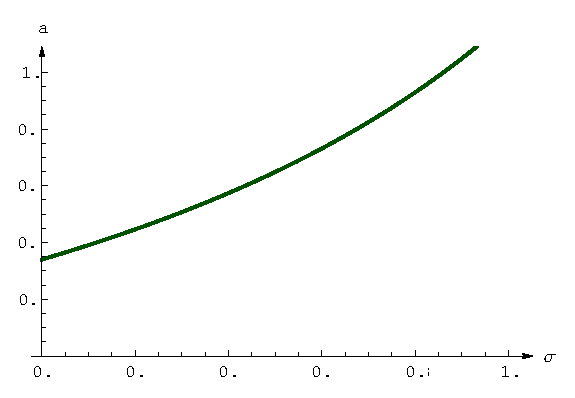
\includegraphics[width=0.47\textwidth]{images/Abbildungen/ATildeR1Ex.eps}}
%		\subfigure[Innovationsstrategie]{%
%		\centering%
%		\psfrag{a}{\small{$\widetilde{a}$}}%
%		\psfrag{0.0}[c]{\scriptsize{0}}%
%		\psfrag{0.2}[c]{\scriptsize{0.2}}%
%		\psfrag{0.4}[c]{\scriptsize{0.4}}%
%		\psfrag{0.6}[c]{\scriptsize{0.6}}%
%		\psfrag{0.8}[c]{\scriptsize{0.8}}%
%		\psfrag{1.0}[c]{\scriptsize{1}}%
%		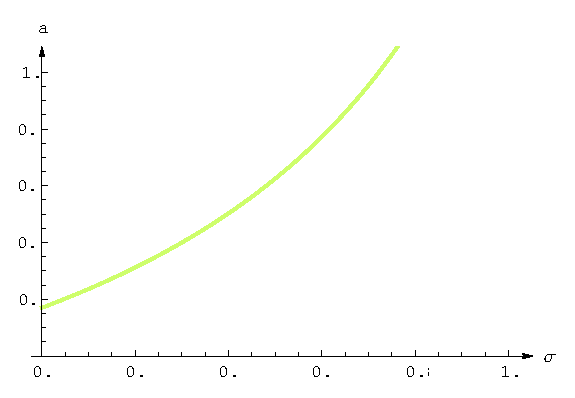
\includegraphics[width=0.47\textwidth]{images/Abbildungen/ATildeR0Ex.eps}}\\
%		\hfill\footnotesize\sffamily{\textbf{Quelle:}}  eigene Darstellung
%		\caption{$\widetilde{a}$ von der Projektgrö{\ss}e} 
%		\label{fig:aTilde}
%	\end{figure}


Die Abbildung \ref{fig:aTilde} zeigt den Zusammenhang zwischen der Nicht-Konvergenz-Falle und der Projektgrö{\ss}e $\sigma$, separat für jede Strategie. Im wesentlichen verhalten sich die Grenzwerte $\tilde{a}$ beider Strategien sehr ähnlich, da beide mit zunehmender Projektgrö{\ss}e ansteigen. Jedoch steigt der Grenzwert der \textcolor[rgb]{0.74,0.97,0.22}{Innovationsstrategie} etwas steiler an, demnach liegt die Nicht-Konvergenz-Falle bei der jeweiligen Projektgrö{\ss}e bei einem höheren Entwicklungsstand als bei der \textcolor[rgb]{0,0.32,0}{Imitationsstrategie}. Mit zunehmender Grö{\ss}e der Projekte kann die Nicht-Konvergenz-Falle durch Verwirklichung der \textcolor[rgb]{0.74,0.97,0.22}{Innovationsstrategie} verzögert werden und somit ein höherer maximal erziehlbarer Entwicklungsstand verwirklicht werden. Jedoch ist dieser Zusammenhang nicht allgemeingültig, wie die folgende Abbildung \ref{fig:beide Strategien mitaTilde} zeigt. \\


	\begin{figure*}[htbp]
		\vspace{0.13cm}
		\centering
		\psfrag{\sigma}{$\sigma$}
		\psfrag{a}{$\widetilde{a}$}
		\psfrag{0.0}[c]{\scriptsize{0}}
		\psfrag{0.2}[c]{\scriptsize{0.2}}
		\psfrag{0.4}[c]{\scriptsize{0.4}}
		\psfrag{0.6}[c]{\scriptsize{0.6}}
		\psfrag{0.8}[c]{\scriptsize{0.8}}
		\psfrag{1.0}[c]{\scriptsize{1}}
		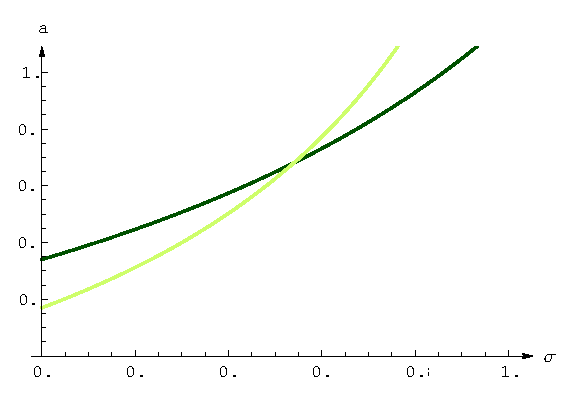
\includegraphics[width=0.7\textwidth]{images/Abbildungen/beideATildeInEinerAbbEx.eps}\\
		\hfill\footnotesize\sffamily{\textbf{Quelle:}}  eigene Darstellung
		\caption{beide Strategien mit $\widetilde{a}$}
		\label{fig:beide Strategien mitaTilde}
	\end{figure*}


Denn der Schnittpunkt beider Geraden gibt an, ab wann die \textcolor[rgb]{0.74,0.97,0.22}{Innovationsstrategie} zu einer Verzögerung der Nicht-Konvergenz-Falle beiträgt. Bis zu diesem Punkt kann durch die \textcolor[rgb]{0,0.32,0}{Imitationsstrategie} ein höherer maximaler technologischer Entwicklungsstand erreicht werden. Diese Möglichkeit ist in Abbildung \ref{fig:ein Sektor exogene WTG} dargestellt und die Volkswirtschaft erreicht den maximal erzielbaren Entwicklungsstand bevor ein Strategiewechsel bedingt durch $a_r$ ratsam wäre.\\


Der maximal erzielbare Wissensstand $\tilde{a}$ sinkt im Importsektor  und steigt im Exportsektor durch den staatlichen Eingriff an, wie aus den Abbildungen \ref{fig:exogene WTG Importsektor} und \ref{fig:exogene WTG Exportsektor} abzulesen ist. Im \textbf{Importsektor} wird dann die Nicht-Konvergenz-Falle $\tilde{a}_{Autarkie}$ nicht mehr durch die Innovation erzielt, sondern durch die \textcolor[rgb]{0,0.32,0}{Imitationsstrategie} bei $\tilde{a}_{Handel}$, da $a_{rHandel}>\tilde{a}_{Handel}$. In der Autarkiesituation lag der Grenzwert bei $a_{rAutarkie}<\tilde{a}_{rAutarkie}$, was den erfolgten Wechsel zur \textcolor[rgb]{0.74,0.97,0.22}{Innovationsstrategie} bedingt. Wohingegen im \textbf{Exportsektor} eine deutliche Verbesserung des maximal erzielbaren Wissenstandes $\tilde{a}$ durch Au{\ss}enhandel erreicht werden kann mit $\tilde{a}_{Autarkie}<\tilde{a}_{Handel}$.\\
Welche Strategie vorherrscht und die Nicht-Konvergenz-Falle eines Sektors bedingt hängt ma{\ss}geblich von der Projektgrö{\ss}e ab. Ab einer kritischen Projektgrö{\ss}e $\overline{\sigma}$ wird die Nicht-Konvergenz-Falle bei der Innovationsstrategie liegen. Dieser Wert ergibt sich aus dem Schnittpunkt beider Geraden von $\tilde{a}$ in Abbildung \ref{fig:beide Strategien mitaTilde} bzw. aus der Gleichsetzung der Gleichungen \ref{eq:aTilde1} und \ref{eq:aTilde0}.


	\begin{equation} 
		\overline{\sigma}=\frac{2+2g-\lambda\gamma}{2+2g+\lambda\gamma}
	\end{equation} 


Immer, wenn $\sigma>\overline{\sigma}$ gilt, dann fand bereits ein Wechsel bedingt durch $a_r$ statt, weil ebenfalls gilt, dass $a_r<\tilde{a}_{Imitation}$. Der maximal erzielbare Entwicklungsstand wird durch die Innovationsstrategie festgelegt. Wohingegen die Imitationsstrategie den maximalen Entwicklungsstand bildet, wenn der Grenzwert $a_r$ noch nicht überschritten wurde und somit für das Projekt gelten muss, dass $\sigma<\overline{\sigma}$.\\
Jedoch ist es durchaus denkbar, dass die Position einer Volkswirtschaft sich verändert. Im Zuge des Entwicklungsprozesses kann ein Land in stark spezialisierten Märkten Makroinnovationen entwickeln und damit den Einfluss eines technologisch gro{\ss}en Landes haben. Die Nicht-Konvergenz-Falle gibt somit nicht zwingend das finale Entwicklungspotenzial eines Landes an. 


\subsection{Wirkung von Handel auf das technologisch gro{\ss}e Land}
Eine Exportsubvention im hier beschriebenen Sinne hat auf den Abstand zur WTG eines ökonomisch gro{\ss}en Landes eindeutige gleichgerichtete Effekte. Die WTG steigt gemeinsam mit dem technischen Wissen und wird durch einen Anstieg der Projektgrö{\ss}e positiv beeinflusst. Die WTG verhält sich somit endogen.  
Anhand der Abbildungen \ref{fig:endogene WTG Importsektor} und \ref{fig:endogene WTG Exportsektor} lassen sich die Reaktionen der Sektoren auf die handelspolitische Ma{\ss}nahme verdeutlichen.\\


	\begin{figure}[htb]
		\vspace{0.13cm}
		\centering 
		\psfrag{a}{$a$}
		\psfrag{t}{  $_t$}
		\psfrag{-}{  $_-$}
		\psfrag{1}{\, $_1$}
		\psfrag{0.0}[c]{\scriptsize{0}}
		\psfrag{0.2}[c]{\scriptsize{0.2}}
		\psfrag{0.4}[c]{\scriptsize{0.4}}
		\psfrag{0.6}[c]{\scriptsize{0.6}}
		\psfrag{0.8}[c]{\scriptsize{}}
		\psfrag{1.0}[c]{\scriptsize{1}}
		\begin{overpic}
			[width=0.9\textwidth]{images/Abbildungen/ImEndogeneWTG.eps}
			\put(73.2,0.5){\textcolor{black}{$\hat{a}_{tAutarkie}$}}
			\put(23,0.7){\textcolor{black}{$a_{rAutarkie}$}}
			\put(60.3,0.7){\textcolor{black}{$a_{rHandel}$}}
			\put(-0.4,45.5){\textcolor{black}{\scriptsize{0.8}}}
			\put(92,0.5){\textcolor{black}{\scriptsize{1}}}
		\end{overpic}\\
		\hfill\footnotesize\sffamily{\textbf{Quelle:}}  eigene Darstellung
		\caption{endogene WTG im Importsektor}
		\label{fig:endogene WTG Importsektor}
	\end{figure}


Beginnend mit dem \textbf{Importsektor} aus Abbildung \ref{fig:endogene WTG Importsektor} führt die Exportsubvention zu verhältnismä{\ss}ig kleineren Projekte im Vergleich zur Autarkiesituation. Insgesamt kann sich der Wissenszuwachs des Importsektors erhöhen indem die \textcolor[rgb]{0,0.32,0}{Imitationsstrategie} verfolgt wird. Die \textcolor[rgb]{0.74,0.97,0.22}{Innovationsstrategie} würde nun zu einem geringeren Entwicklungsstand führen, was wiederum eindeutig zeigt, dass der Importsektor seinen Schwerpunkt auf langfristige Beziehungen, die Ausdruck der \textcolor[rgb]{0,0.32,0}{Investitionsstrategie} sind, legen sollte. Die Grenzwerte $a_r$ und $\hat{a}_t$ steigen beide mit sinkender Projektgrö{\ss}e und deuten an, dass sowohl hinsichtlich der Produktivität $\hat{a}_{tHandel}>1$ als auch der Wirtschaftlichkeit $a_{rHandel}>a_{rAutarkie}$ ein späterer Wechsel zur \textcolor[rgb]{0.74,0.97,0.22}{Innovationsstrategie} zu empfehlen ist. Der Sektor ist vornehmlich durch die \textcolor[rgb]{0,0.32,0}{Imitationsstrategie} geprägt. Die kleinen Importprojekte verlieren bei der strategischen Planung zunehmend an Bedeutung, da die unternehmerischen Umsätze durch die sehr kleinen Projekte verglichen mit den gesamtwirtschaftlichen Umsätzen nur einen relativ geringen Anteil betragen. Bleibt die Angestelltenstruktur gemä{\ss} der \textcolor[rgb]{0,0.32,0}{Imitationsstrategie} unverändert, dann liegt der Schwerpunkt bei den gro{\ss}en Projekten, die durch die weniger gut ausgebildeten erfahrenen Ingenieure ermöglicht werden.\\ Interessant ist ein Vergleich von Volkswirtschaften deren Entwicklungsstand nur geringfügig grö{\ss}er oder kleiner als $a_{rHandel}$ ist. Da je nach Startsituation das relativ weiter entwickelte Land mit $a_{t-1}>a_{rHandel}$ von dem weniger weit entwickelten Land $a_{t-1}<a_{rHandel}$ durch den Wechsel zur \textcolor[rgb]{0.74,0.97,0.22}{Innovationsstrategie} überholt werden kann.\\


	\begin{figure}[htb]
		\vspace{0.13cm}
		\centering 
		\psfrag{a}{$a$}
		\psfrag{t}{  $_t$}
		\psfrag{-}{  $_-$}
		\psfrag{1}{\, $_1$}
		\psfrag{0.0}[c]{\scriptsize{0}}
		\psfrag{0.2}[c]{\scriptsize{}}
		\psfrag{0.4}[c]{\scriptsize{0.4}}
		\psfrag{0.6}[c]{\scriptsize{0.6}}
		\psfrag{0.8}[c]{\scriptsize{}}
		\psfrag{1.0}[c]{\scriptsize{1}}
		\begin{overpic}
			[width=0.9\textwidth]{images/Abbildungen/ExEndogeneWTG.eps}
			\put(25,0.5){\textcolor{black}{$\hat{a}_{tHandel}$}}
			\put(71.6,0.5){\textcolor{black}{$\hat{a}_{tAutarkie}$}}
			\put(22.4,-1.6){\textcolor{black}{$a_{rAutarkie}$}}
			\put(-0.73,13.3){\textcolor{black}{\scriptsize{0.2}}}
			\put(-0.73,45){\textcolor{black}{\scriptsize{0.8}}}
		\end{overpic}\\
		\hfill\footnotesize\sffamily{\textbf{Quelle:}}  eigene Darstellung
		\caption{endogene WTG im Exportsektor}
		\label{fig:endogene WTG Exportsektor}
	\end{figure}


Im \textbf{Exportsektor} in Abbildung \ref{fig:endogene WTG Exportsektor} verhält es sich etwas anders. Grundsätzlich führt eine grö{\ss}ere Projektgrö{\ss}e zu einem höheren Wissenszuwachs durch die \textcolor[rgb]{0.74,0.97,0.22}{Innovationsstrategie} und zu einer Wissensreduktion, sollte sich der Sektor nach der \textcolor[rgb]{0,0.32,0}{Investitionsstrategie} ausrichten. Auch im Exportsektor hängt die Wahl der Strategie vom Entwicklungsstand eines Landes ab. Für weniger weit entwickelte Länder ist die \textcolor[rgb]{0,0.32,0}{Imitationsstrategie} noch immer produktiver als die \textcolor[rgb]{0.74,0.97,0.22}{Innovationsstrategie}, jedoch führt sie zu einem geringeren Wissenszuwachs als dies \dashuline{ohne Handelspolitik} möglich wäre. Bei der endogenen WTG führt die \uline{Exportsubvention} allgemein zu einer relativ schlechteren Produktivität. Der Entwicklungspfad eines Landes wird nicht uneingeschränkt von der staatlichen Unterstützung beschleunigt, jedoch werden die Innovationen in diesem Sektor gefördert und ein früherer Wechsel zur \textcolor[rgb]{0.74,0.97,0.22}{Innovationsstrategie} ist sinnvoll. Die Exportförderung wirkt ähnlich wie eine Förderung von Unternehmensgründungen, da diese sofern sie sich im Exportsektor ansiedeln, eine solidere und sicherere Ausgangssituation vorfinden, als ohne unterstützende Ma{\ss}nahmen.\\


Werden wieder die Schwellenwerte $a_r$ und $\hat{a}_t$ hinzugezogen, dann sinken beide Werte mit steigender Projektgrö{\ss}e. Da hier $a_{rHandel}<0$ gilt, ist es ökonomisch sinnvoll nur noch die \textcolor[rgb]{0.74,0.97,0.22}{Innovationsstrategie} zu verfolgen. Durch die Exportsubvention stellen sich nur Länder mit einem Entwicklungsstand $a_{t-1}>a_{rAutarkie}$ besser.\\


Die Nicht-Konvergenz-Falle $\tilde{a}$ ist auch bei Handel bei der endogenen WTG nicht relevant, da alle Volkswirtschaften sich im Entwicklungsprozess zur Innovationsstrategie ausrichten und dann zur WTG mit $\tilde{a}=1$ konvergieren. 


\section{Zwischenfazit}
Das vorliegende Wachstumsmodell zeigt, inwiefern  Handel die technische Entwicklung eines Landes fördert. Um die Ergebnisse zu verdeutlichen, wurde eine handelsfördernde Ma{\ss}nahme eingeführt und es lassen sich Entwicklungsstrategien für verschiedene Entwicklungsphasen zuordnen. Neben dem Entwicklungsstand eines Landes wurde auch die Bedeutung einer Innovation für das Land miteinbezogen.\\
Zusammenfassend lässt sich festhalten, dass ökonomisch und technologisch kleine Länder bei einer exogenen WTG von einer Exportförderung profitieren. Im Exportsektor kann es zu einer deutlichen Verbesserung des technischen Entwicklungsstandes kommen und der Abstand zur WTG mindert sich eher, als dies ohne Exportförderung möglich ist, unabhängig von dem technologischen Entwicklungsstand eines Landes.\footnote{Siehe dazu auch Abbildung \ref{fig:exogene WTG Exportsektor}.} Es findet eine eindeutige Verlagerung des Schwerpunktes dieses Sektors zur Innovationsstrategie statt. Wohingegen der Importsektor sich ausschlie{\ss}lich auf die Imitationsstrategie konzentriert. Dabei stellen sich relativ wenig entwickelte Länder sowie auch deutlich weiter entwickelte Länder mit der Exportsubvention schlechter und sollten auf Au{\ss}enhandel in diesem Sektor zunächst verzichten. In diesem, hier angenommenen, Fall profitiert der Importsektor nur in wenigen Fällen vom Au{\ss}enhandel. Demnach verschlechtert sich das allgemeine Entwicklungspotential $\tilde{a}$ dieses Sektors durch Handel. Jedoch kann insgesamt von einer Verbesserung durch Handel ausgegangen werden.\\


	\begin{figure}[h!] 
		\vspace{0.13cm}
		\centering 
		\psfrag{a}{$a$}
		\psfrag{t}{  $_t$}
		\psfrag{-}{  $_-$}
		\psfrag{1}{\, $_1$}
		\psfrag{0.0}[c]{\scriptsize{0}}
		\psfrag{0.2}[c]{\scriptsize{0.2}}
		\psfrag{0.4}[c]{\scriptsize{}}
		\psfrag{0.6}[c]{\scriptsize{0.6}}
		\psfrag{0.8}[c]{\scriptsize{0.8}}
		\psfrag{1.0}[c]{\scriptsize{1}}
		\begin{overpic}	[width=0.9\textwidth]{images/Abbildungen/beideSektorenExoWTG.eps}
			\put(35.9,0.7){\color[rgb]{0,0.32,0}{$\tilde{a}_{Im}$}}
			\put(59.2,0.7){\color[rgb]{0.74,0.97,0.22}{$\tilde{a}_{Ex}$}}
			\put(-0.73,24.2){\textcolor{black}{\scriptsize{0.4}}}
		\end{overpic}\\
		\hfill\footnotesize\sffamily{\textbf{Quelle:}}  eigene Darstellung
		\caption{beide Sektoren bei exogener Welttechnologiegrenze}
		\label{fig:beide Sektor exogene WTG}
	\end{figure}


Die gemeinsame Darstellung des Import- mit dem Exportsektor in Abbildung \ref{fig:beide Sektor exogene WTG}\footnote{In der Abbildung sind die Strategien des Exportsektors mit den dickeren Linien gekennzeichnet und die Strategien des Importsektor mit den dünneren Linien.}  zeigt, dass eine Exportförderung in einem technologisch kleinen Land zu einer Konzentration des Importsektors auf die Imitationsstrategie und des Exportsektors auf die Innovationsstrategie führt, unabhängig vom Entwicklungsstand des Landes.Der Vergleich beider Sektoren zeigt eindeutig, dass die Nicht-Konvergenz-Falle im Exportsektor $\tilde{a}_{Ex}$ deutlich später eintritt, als im Importsektor $\tilde{a}_{Im}$ und somit auch einen höheren maximal erzielbaren technologischen Entwicklungsstand erreichen kann, da $\tilde{a}_{Im}<\tilde{a}_{Ex}$ gilt. Die lokale Technologiegrenze wird hier demzufolge eindeutig durch den Exportsektor gebildet und das Land profitiert insgesamt vom Au{\ss}enhandel.\\ 


Bei einer endogenen WTG hingegen verschlechtert sich das Entwicklungspotenzial des Exportsektors teilweise. Unabhängig von dem Entwicklungsstand des Landes wird die Innovationsstrategie verfolgt. Erst ab dem bestimmten technologischen Entwicklungsniveau $a_{rAutarkie}$ stellt sich eine Volkswirtschaft mit einer Exportförderung besser als bei Autarkie.\footnote{Dieser Zusammenhang ist der Abbildung \ref{fig:endogene WTG Exportsektor} zu entnehmen.} Demzufolge sollte sich bis zu diesem Entwicklungsstand die Volkswirtschaft nicht für Handel öffnen, sofern nur der Exportsektor betrachtet wird. Denn der Zuwachs des gesamtwirtschaftlichen technischen Wissens bestimmt sich durch die vorherrschende Imitationsstrategie im Importsektor. In diesem Sektor sollte jedoch wieder differenziert werden hinsichtlich des Entwicklungsstandes und der Öffnung für Au{\ss}enhandel. Sofern ein Land recht weit entwickelt ist und den Grenzwert $a_{rHandel}$ bereits überschritten hat verschlechtern sich die Entwicklungsmöglichkeiten im Importsektor. Letztlich verbessert sich die gesamte Volkswirtschaft durch Au{\ss}enhandel, im endogenen Fall jedoch ist dies grö{\ss}tenteils auf den Importsektor zurückzuführen.\footnote{Zu finden sind diese Grenzwerte in Abbildung \ref{fig:endogene WTG}} 
		
			
	\begin{figure}[h!] 
		\vspace{0.13cm}
		\centering  
		\psfrag{a}{$a$}
		\psfrag{t}{  $_t$}
		\psfrag{-}{  $_-$}
		\psfrag{1}{\, $_1$}
		\psfrag{0.0}[c]{\scriptsize{0}}
		\psfrag{0.2}[c]{\scriptsize{0.2}}
		\psfrag{0.4}[c]{\scriptsize{0.4}}
		\psfrag{0.6}[c]{\scriptsize{0.6}}
		\psfrag{0.8}[c]{\scriptsize{0.8}}
		\psfrag{1.0}[c]{\scriptsize{1}}
		\begin{overpic}[width=0.9\textwidth]{images/Abbildungen/beide.eps}
			\put(58.2,0.9){\textcolor{black}{$a_{rIm}$}}
		\end{overpic}\\
		\hfill\footnotesize\sffamily{\textbf{Quelle:}}  eigene Darstellung
		\caption{beide Sektoren bei endogener Welttechnologiegrenze}
		\label{fig:beideSektorenendogeneWTG}
	\end{figure}


In der zweiten sektorübergreifenden Darstellung \ref{fig:beideSektorenendogeneWTG}\footnote{Auch hier können die Sektoren wieder anhand der Dicke der Linien unterschieden werden: Die Strategien des Exportsektors sind mit den dickeren Linien gekennzeichnet und die Strategien des Importsektor mit den dünneren Linien.} liegt der Schwerpunkt des Exportsektors ebenfalls in der Innovationsstrategie, wohingegen beim Importsektor ab einem bestimmten technologischen Entwicklungsstand von $a_{rIm}$ die weniger produktive Innovationsstrategie gewählt wird. Bis zu diesem Schwellenwert bildet der Importsektor den lokalen technologischen Wissensstand der Volkswirtschaft ab und bedingt dadurch stärker den technischen Fortschritt als der innovierende Exportsektor.\newline 
Zusammenfassend lässt sich feststellen, dass in technologisch kleinen Ländern unabhängig von dem Entwicklungsstand im Importsektor die Imitationsstrategie und im Exportsektor die Innovationsstrategie verfolgt wird. Es stellen sich Länder aller Entwicklungsstufen besser durch eine Exportsubvention. In technologisch gro{\ss}en Ländern profitieren ebenfalls alle Länder, unabhängig vom technologischen Entwicklungsstand, von der Förderung des Exportsektors. 


\chapter{Kombination beider Modellvarianten}\label{Kombi}
Anhand der bisherigen Ergebnisse konnte festgestellt werden, dass sich die Entscheidung
der Haushalte zwischen der eigenen Bildung oder der Erwerbstätigkeit durch die Integration vom Au{\ss}enhandel zugunsten der Weiterbildung verlagerte. Hebt man dieses Ergebnis auf die makroökonomische Ebene, dann kann insgesamt von einer besser ausgebildeten Gesellschaft ausgegangen werden. Die Öffnung eines Landes führt dazu, dass mehr Humankapitel akkumuliert wird. Dieses zusätzliche Humankapital kann nun verwendet werden, um den technischen Fortschritt durch Imitation oder Innovation in einem Land zu steigern. Das zuvor behandelte Modell in Kapitel \ref{Papier2} stellt somit den notwendigen vorgelagerten Prozess dar, durch den es erst möglich wird den technischen Entwicklungsstand eines Landes zu verbessern, was in Kapitel \ref{Papier1} umfasend analysiert wurde.\newline 
Das folgende Kapitel soll nun die Wahrscheinlichkeit einer guten Ausbildung eines Ingenieurs $\lambda$ genauer betrachten.\footnote{Dabei wird nun, ohne Verlust von Allgemeinheit, von einer exogenen Projektgrö{\ss}e ausgegangen.} Durch den gezeigten positiven Zusammenhang von Au{\ss}enhandel und Investitionen in Bildung steigt nun ebenfalls die Wahrscheinlichkeit, dass ein Ingenieur mit hohen technischen Fähigkeiten ausgestattet ist, denn ein grundlegend angepasstes und in diesem Fall verbessertes Bildungssystem führt zu einer besser ausgebildeten Bevölkerung. Somit steigt in diesem Fall auch die Wahrscheinlichkeit einen gut ausgebildeten Ingenieur einzustellen an, als dies ohne Handel der Fall wäre.  \\
Ohne, dass der Handel explizit politisch unterstützt wurde, verbessert sich der technologische Entwicklungsstand eines Landes. Auch dies ist wieder abhängig von der strategischen Entscheidung eines Unternehmens bzw. der Volkswirtschaft. Die folgende Abbildung \ref{lambdaExo} stellt den Vergleich der beiden Strategien einer geöffneten und einer geschlossenen Volkswirtschaft dar.\\


	\begin{figure}[htbp] 
		\vspace{0.13cm}
		\centering  
		\psfrag{a}{$a$}
		\psfrag{t}{  $_t$}
		\psfrag{-}{  $_-$}
		\psfrag{1}{\, $_1$}
		\psfrag{0.0}[c]{\scriptsize{0}}
		\psfrag{0.2}[c]{\scriptsize{0.2}}
		\psfrag{0.4}[c]{\scriptsize{0.4}}
		\psfrag{0.6}[c]{\scriptsize{0.6}}
		\psfrag{0.8}[c]{\scriptsize{0.8}}
		\psfrag{1.0}[c]{\scriptsize{1}}
		\begin{overpic}[width=0.9\textwidth]{images/Abbildungen/Lambdaaexo.eps}
			\put(47,-0.93){\textcolor{black}{$\hat{a}_{t\textit{Handel}}$}}
			\put(74.5,-0.86){\textcolor{black}{$\hat{a}_{t\textit{Autarkie}}$}}
			\put(14.3,-1.1){\textcolor{black}{$a_{rHandel}$}}
			\put(21.7,0.5){\textcolor{black}{$a_{rAutarkie}$}}
		\end{overpic}\\
		\hfill\footnotesize\sffamily{\textbf{Quelle:}}  eigene Darstellung
		\caption{Einfluss der Wahrscheinlichkeit für qualifizierte Arbeit $\lambda$ bei exogener WTG auf den technologischen Entwicklungsstand}
		\floatfoot{- Anstieg der Wahrscheinlichkeit für qualifizierte Arbeit $\lambda$ von 50\% auf 80\% durch Freihandel -}
		\label{lambdaExo}
	\end{figure}


Von einer geschlossenen Volkswirtschaft ausgehend, die weitestgehend autark ist, steigt in dem hier dargestellten Fall die Wahrscheinlichkeit einen Ingenieur eingestellt zu haben, der hohe technische Fähigkeiten besitzt von 50\% auf 80\% an. Füt den technologischen Entwickungsstand eines Landes bedeutet dies, dass hierdurch ein höherer zukünftiger Zustand erreicht werden kann, für jeden technologischen Entwicklungsstand eines Landes. Die Geraden verlaufen steiler und dementsprechend führt dies unabhängig von der Strategiewahl zu einem zusätzlichen Wachstum, denn je besser ausgebildet die Arbeiter sind, desto mehr Wissen kann transferiert werden und die entsprechenden Volkswirtschaften profitieren durch diese Wissens-Spillover-Effekte.\\ 
Der Grenzwert $\hat{a}$ betrachtet den Strategiewechsel losgelöst von möglichen Kosten und sinkt mit zunehmendem Handel. Auf die Entwicklung eines Landes bezogen wird nun schon für Länder mit einem geringeren technologischem Entwicklungsstand der Wechsel zur \textcolor[rgb]{0.74,0.97,0.22}{Innovationsstrategie} empfohlen, da diese produktiver ist. In einer \dashuline{geschlossenen Volkswirtschaft}, in der von einem geringeren Kapitalstock ausgegangen werden kann, dominierte die \textcolor[rgb]{0,0.32,0}{Imitationsstrategie}. Mit der \underline{Öffnung des Landes} resultiert grundsätzlich ein deutlich höherer technologischer Entwicklungsstand, der zunächst eher durch die \textcolor[rgb]{0,0.32,0}{Imitationsstrategie} erzielt werden kann.  Der höhere Entwicklungsstand ergibt sich durch besser ausgebildete Arbeiter, die nun vorhanden sind. Für innovierende Tätigkeiten sind hohe technische Fähigkeiten notwendig, die fortan eingesetzt werden können und die Innovationsrate steigern.\\
Berücksichtigt man die Gewinnaussichten der Unternehmer, dann zeigt auch der Grenzwert $a_r$, dass Offenheit zu einem früheren Wechsel zur Innovationsstrategie führt. \\


	\begin{figure*}[h]
		\vspace{0.13cm}
		\centering
		\psfrag{a}{$a_r$}
		\psfrag{t}{}
		\psfrag{-}{-}
		\psfrag{1}{1}
		%\psfrag{-0.2}[c]{\scriptsize{}}
		%\psfrag{-0.4}[c]{\scriptsize{}}
		\psfrag{0.0}[c]{\scriptsize{0}}
		\psfrag{0.2}[r]{\scriptsize{0.2}}
		\psfrag{0.4}[r]{\scriptsize{0.4}}
		\psfrag{0.6}[r]{\scriptsize{0.6}}
		\psfrag{0.8}[r]{\scriptsize{0.8}}
		\psfrag{1.0}[r]{\scriptsize{1}}
		\psfrag{L}[c]{$\lambda$}
		\begin{overpic}[width=0.5\textwidth]{images/Abbildungen/aRLambda.eps}
			%\put(98,16){\textcolor{black}{$\sigma$}}
			%\put(0.5,23){\textcolor{black}{\scriptsize{0.2}}}
			%\put(0.5,30){\textcolor{black}{\scriptsize{0.4}}}
			%\put(0.5,38){\textcolor{black}{\scriptsize{0.6}}}
			%\put(0.5,45.1){\textcolor{black}{\scriptsize{0.8}}}
			
			%\put(20.6,12){\textcolor{black}{\scriptsize{0.2}}}
			%\put(38.4,12){\textcolor{black}{\scriptsize{0.4}}}
			%\put(56.2,12){\textcolor{black}{\scriptsize{0.6}}}
			%\put(74.3,12){\textcolor{black}{\scriptsize{0.8}}}
		\end{overpic}\\
		\hfill\footnotesize\sffamily{\textbf{Quelle:}}  eigene Darstellung
		\caption{$a_r$ in Abhängigkeit von $\lambda$ }
		\label{fig:VerhaltenAR}
	\end{figure*}


Sofern die Wahrscheinlichkeit ansteigt, dass ein junger Ingenieur hohe technische Fähigkeiten besitzen könnte, werden diese Möglichkeiten von den Unternehmen erkannt und es findet ein früherer Wechsel der Strategie statt, da ein geringerer Wert von $a_r$ folgt. Kurze berufliche Beziehungen werden präferiert und ältere  weniger qualifizierte Ingenieure ausgetauscht, wodurch die Kosten reduziert werden. Dieses Modell zeigt direkt, dass Ineffizienzen beseitigt bzw. gemindert werden, indem das Risiko eingegangen wird junge Ingenieure einzustellen, die möglicherweise höher qualifiziert sind.
In diesem Zusammenhang führt Handel zu tendenziell mehr Entlassungen weniger qualifizierter Ingenieure und zu einem Anstieg der Innovationsrate.\\
Anzumerken ist an dieser Stelle, dass bei relativ weiter entwickelten Volkswirtschaften, die in Relation zur WTG mit mindestens 80\% entwickelt sind, beide Strategien in Abbildung \ref{fig:beideSektorenendogeneWTG} nicht definiert sind. Bei diesen Ländern kann davon ausgegangen werden, dass sie nach dem Wechsel zur Innovationsstrategie keine Mikro- sondern Makroinnovationen entwickeln und somit als technologisch gro{\ss}es Land selbst die WTG dieser Branche stellen. Dann handelt es sich um eine endogene WTG, die in der folgenden Abbildung \ref{lambdaEndo} dargestellt ist.\\


	\begin{figure}[htbp] 
		\vspace{0.13cm}
		\centering  
		\psfrag{a}{$a$}
		\psfrag{t}{  $_t$}
		\psfrag{-}{  $_-$}
		\psfrag{1}{\, $_1$}
		\psfrag{0.0}[c]{\scriptsize{0}}
		\psfrag{0.2}[c]{\scriptsize{0.2}}
		\psfrag{0.4}[c]{\scriptsize{0.4}}
		\psfrag{0.6}[c]{\scriptsize{0.6}}
		\psfrag{0.8}[c]{\scriptsize{}}
		\psfrag{1.0}[c]{\scriptsize{1}}
		\begin{overpic}[width=0.9\textwidth]{images/Abbildungen/Lambdaaendo.eps}
			\put(44.5,0.7){\textcolor{black}{$\hat{a}_{t\textit{Handel}}$}}
			\put(73,0.7){\textcolor{black}{$\hat{a}_{t\textit{Autarkie}}$}}
			\put(-1,45.5){\textcolor{black}{\scriptsize{0.8}}}
			%\put(-0.5,55.5){\textcolor{black}{\scriptsize{1}}}
			\put(13,-1){\textcolor{black}{$a_{rHandel}$}}
			\put(21.5,0.7){\textcolor{black}{$a_{rAutarkie}$}}
		\end{overpic}\\
		\vspace{0.3cm}
		\hfill\footnotesize\sffamily{\textbf{Quelle:}}  eigene Darstellung
		\caption{Einfluss der Wahrscheinlichkeit für qualifizierte Arbeit $\lambda$ bei endogener WTG auf den technologischen Entwicklungsstand}
		\floatfoot{- Anstieg der Wahrscheinlichkeit für qualifizierte Arbeit $\lambda$ von 50\% auf 80\% durch Freihandel -}
		\label{lambdaEndo}
	\end{figure}


Auch hier wird von einer staatlichen Exportförderung abstrahiert und einzig der Effekt des Au{\ss}enhandels durch höhere Bildung auf den Entwicklungsstand eines Landes betrachtet. In einem technologisch gro{\ss}en Land weitet sich die WTG mit jeder zusätzlichen Innovation aus.\\ Ist dieses Land \underline{offen}, dann entsteht zunächst der Eindruck, dass es seinen direkten Wissensvorsprung gegenüber der übrigen Welt verliert. Abbildung \ref{lambdaEndo} stellt dar, dass sich der technologische Entwicklungsstand eines Landes durch Au{\ss}enhandel, unabhängig von dem anfänglichen Entwicklungsstand verschlechtert. Dieser Anschein wird durch die relative Darstellung des Entwicklungsstandes hervorgerufen.\footnote{Dies ergibt sich durch die Definition des Abstands zur Welttechnologiegrenze eines Landes $a_t$ als $A_t/\bar{A_t}$.} Der Entwicklungsstand eines Landes steigt bei einer endogenen WTG nur dann an, wenn es selbst einen stärkeren technologischen Wissenszuwachs generiert, als das Land, welches die Technologiegrenze erweitert hat. Dass hierdurch Au{\ss}enhandel die Wahrscheinlichkeit steigt qualifizierte Arbeitskräfte einzustellen, steigert die Produktivität eines Landes und führt zu Wachstum. Jedoch ist die Produktivität des Landes der WTG noch immer höher und die Ausweitung der WTG ist stärker als die Minderung des Abstandes. Diese Argumentation kann auch anhand der in Kapitel \ref{Efekkte} diskutieren Effekte gestützt werden. Es wurde gezeigt, dass Handel zu einem Produktivitätszuwachs durch den Marktgrö{\ss}eneffekt, den Wettbewerbseffekt und den Wissens-Spillover-Effekt führt. Dieser positiv wirkende Effizienzeffekt wird hier durch den negativ wirkenden Wachstumseffekt dominiert. Der Wachstumseffekt spiegelt das Wachstum der WTG wieder, das den relativen Abstand ausweitet.\footnote{Der Wachstumseffekt resultiert aus der Endogenität der WTG und muss somit nur im endogenen Fall untersucht werden. Bei einer exogenen WTG ist demzufolge immer der Effizienzeffekt dominant.} In der hier dargestellten Situation profitieren vom Au{\ss}enhandel sowohl Unternehmen, die, die \textcolor[rgb]{0.74,0.97,0.22}{Innovationsstrategie} nutzen, als auch die die die \textcolor[rgb]{0,0.32,0}{Imitationsstrategie} verfolgen, jedoch profitiert das Land der WTG stärker, so dass der technologische Entwicklungsstand sinkt, der relativ zur WTG bemessen wird. Das führt dazu, dass ein technologisch gro{\ss}es Land sich relativ gesehen langsamer entwickelt. Dies kann beispielsweise daran liegen, dass auch das Land der WTG von den Ressourcen, wie Kapital, Arbeit und getätigten Investitionen gleicherma{\ss}en profitiert, wie das Ursprungsland, welches darüber hinaus noch Wissen generiert.\\
Nachdem nun die Aussagekraft der Abbildung interpretiert wurde, lässt sich ein optimaler Entwicklungspfad ableiten. Auch hier steigen die Innovationsanreize und es findet aufgrund der besseren Humankapitalausstattung ein früherer Wechsel zur \textcolor[rgb]{0.74,0.97,0.22}{Innovationsstrategie} statt. Jedoch ist der zukünftige Abstand zur WTG höher als in der \dashuline{Autarkiesituation}. Dieser Wechsel wird sowohl durch einen kleineren Grenzwert von $\hat{a}$ als auch von $a_r$ angezeigt.
\bigskip


Zusammenfassend lässt sich feststellen, dass Volkswirtschaften stärker von der Imitationsstrategie profitieren, sofern ihre Mikroinnovationen die WTG nicht tangieren. Erst mit zunehmender Bedeutung der Innovationen folgen die Länder der Innovationsstrategie, die den technologischen Entwicklungsprozess fördert, auch wenn der relative Abstand zur WTG dabei nicht sinkt. \\
Somit wird in dieser Arbeit das tatsächliche Verhalten vieler Länder wiedergespiegelt, die ihren Schwerpunkt auf die Imitation legen. Nur wenige sehr weit entwickelte Länder fokussieren sich auf Innovationen. Viele von ihnen sind meist auch technologisch gro{\ss} und somit führend in ihrer Branche. Durch Au{\ss}enhandel kann insgesamt ein höheres Niveau an Bildung erreicht werden. Demzufolge wird nicht nur besser und mehr innoviert, sondern auch imitiert.